\documentclass{article}
\usepackage[margin=2.5cm, includefoot, footskip=30pt]{geometry}

\setlength{\parindent}{0em}
\setlength{\parskip}{1em}
\renewcommand{\baselinestretch}{1}

%%%%Packages%%%%
\usepackage{amsmath}
\usepackage{booktabs}
\usepackage{graphics}
\usepackage{multicol}
\usepackage[ruled,vlined]{algorithm2e}
\usepackage{setspace}
\usepackage{graphicx}
\usepackage{subcaption}
\usepackage{hyperref}
\usepackage{color,colortbl}
\usepackage{array}
\usepackage{booktabs}
\usepackage{tabularx}
\usepackage{wrapfig, blindtext}
\usepackage[table]{xcolor}
%%%%%%%%%%%%%%%%%

\definecolor{Gray}{gray}{0.92}
\usepackage[first=0,last=9]{lcg}
\newcommand{\ra}{\rand0.\arabic{rand}}

\newcommand{\uniquenumberofseeds}{11400}
\newcommand{\numberofalltournaments}{45606}

\setlength{\tabcolsep}{3pt}

\title{A meta analysis of tournaments and an evaluation of performance in the
Iterated Prisoner's Dilemma.}
\author{Nikoleta E. Glynatsi, Vincent A. Knight}
\date{}

\begin{document}

\maketitle

\begin{abstract}

The Iterated Prisoner's Dilemma has been used for decades as a model of
behavioural interactions. From the celebrated performance of Tit for Tat, to the
introduction of the zero-determinant strategies, to the use of sophisticated
structures such as neural networks, the literature has been exploring the
performance of strategies in the game for years. Most of these strategies are
now accessible due to an open source package; Axelrod-Python. This manuscript
make use of Axelrod-Python to conduct a meta analysis of Iterated Prisoner's
Dilemma tournaments. The aim is to evaluate the performance of 194 strategies
over \numberofalltournaments Iterated Prisoner's Dilemma tournaments and to
explore the factors of their success.
\end{abstract}

\section{Background}

The Iterated Prisoner's Dilemma (IPD) is a repeated two player game that models
behavioural interactions, and more specifically, interactions where
self-interest clashes with collective interest. At each turn of the game both
players, simultaneously and independently, decide between cooperation (C) and
defection (D) whilst having memory of their prior interactions. The payoffs for each
player, at each turn, is influenced by their own choice and the choice of the
other player. The payoffs of the game are generally defined by:

\[\begin{pmatrix}
R & S \\
T & P
\end{pmatrix}\]

where \(T > R > P > S\) and \(2R > T + S\). The most common values used in
the literature~\cite{Axelrod1981} are $R=3, P=1, T=5, S=0$. These values are also
used in this work.

Conceptualising strategies and understanding the best way of playing the game
has been of interest to the scientific community since the formulation of the
game in 1950~\cite{Flood1958}. Following the computer tournaments of Axelrod in the
1980's~\cite{Axelrod1980a, Axelrod1980b}, a strategy's performance in a round
robin computer tournament became a common evaluation technique for newly designed
strategies. Today more than 200 strategies exist in the literature and several
tournaments, excluding Axelrod's, have been undertaken~\cite{Bendor1991,
Harper2017, Kendall2007, Stephens2002, Stewart2012}.

In the 80's, Axelrod performed two computer tournaments~\cite{Axelrod1980a,
Axelrod1980b}. The contestants were strategies submitted in the form of computer
code. They competed against all other entries, a copy of themselves and a random
strategy. The winner was decided on the average score a strategy achieved. The
winner of both tournaments was the simple strategy Tit For Tat which cooperated
on the first turn and then simply copied the previous action of it's opponent.
Due to the strategy's strong performance in both tournaments, and moreover in a
series of evolutionary experiments~\cite{Axelrod1981}, Tit For Tat was thought
to be the most robust basic strategy in the IPD.

However, further research proved that the strategy had weakness, and more
specifically, it was shown that the strategy suffered in environments with
noise~\cite{Bendor1991, Donninger1986, Molander1985, Hammerstein1984}. This was
mainly due to the strategy's lack of generosity and contrition. The strategy was
quick to punish a defection, and in a noisy environment it could lead to a
repeated cycle of defections and cooperations. Some new strategies, more
robust in tournaments with noise, were soon introduced and became the new
protagonists of the game. These include Nice and Forgiving~\cite{Bendor1991},
Pavlov~\cite{Nowak1993} and Generous Tit For Tat~\cite{Nowak1992}.

In 2004, a $20^{\text{th}}$ Anniversary Iterated Prisoner Dilemma Tournament
took place with 233 entries. This time the winning strategy was not designed on
a reciprocity based approach but on a mechanism of
teams~\cite{J.P.Delahaye1993Lp, J.P.Delahaye1995LIeP, A.Rogers2007Ctpw}. A team
from Southampton University took advantage of the fact that a participant was
allowed to submit multiple strategies. They submitted a total of 60 strategies
that could recognised each other and colluded to increase one members score.
This resulted with three of the strategies to be ranked in the top spots. The
performance of the Southampton University team received mixed attention, though
they had won the tournament as stated in~\cite{us_blog} "technically this
strategy violates the spirit of the Prisoner's Dilemma, which assumes that the
two prisoners cannot communicate with one another".

Another set of IPD strategies that have received a lot of attention
are the zero-determinants~\cite{Press2012}. By
forcing a linear relationship between the payoffs the zero-determinant
strategies can ensure that they will never receive less than their opponents.
The
American Mathematical Society's news section stated that ``the world of game
theory is currently on fire''.
Zero-determinant strategies are indeed a set of mathematically unique strategies
and robust in pairwise interactions, however, their simplicity and extortionate
behaviour have been tested. In~\cite{Harper2017} a tournament containing over
200 strategies, including zero-determinants, was ran. None of the zero-determinant
strategies ranked in top spots. Instead, the top ranked strategies were a set of
trained strategies based lookup tables~\cite{Axelrod1987}, hidden markov
models~\cite{Harper2017} and finite state automata~\cite{Miller1996}.

Though only a select pieces of work have been discussed, the IPD is
rich, and new strategies and competitions are being published every year.
The question, however, still remains the same: what is the best way to play the
game?

This manuscript uses an open source package called
Axelrod-Python~\cite{axelrodproject} to simulate a large number of computer
tournaments, using as many strategies as possible from the literature. The aim
is to evaluate the performance of 194 strategies in IPD tournaments, and
futhermore, explore the factors of their success. This is done not only for
standard round robin tournaments, but also for tournaments with noise and
tournaments with a probabilistic ending. The different tournament types as well
as the data collection are covered in Section~\ref{section:data_collection}.
Section~\ref{section:top_performances}, focuses on the best performing strategies
for each type of tournament and overall.
Section~\ref{section:evaluation_of_performance}, explores the traits which
contribute to good performance, and finally the results are summarised in
Section~\ref{section:conclusion}.

This manuscripts uses several parameters. These are introduced in the following
sections, however, the full set of parameters and their definitions are given in
Appendix~\ref{app:parameters}. All the data is available at~\cite{data}.

\section{Data collection}\label{section:data_collection}

For the purposes of this manuscript a data set containing results of IPD tournaments
has been generated and is available at~\cite{data}. This
was done using the open source package Axelrod-Python~\cite{axelrodproject}, and
more specifically, version 3.0.0. Axelrod-Python allows for different types of
IPD computer tournaments to be simulated whilst
containing a list of over 180 strategies. Most of these are strategies described
in the literature with a few exceptions being strategies that have been
contributed specifically to the package. This paper make use of 194 strategies
implemented in version 3.0.0. A list of the strategies is given in the
Appendix~\ref{app:list_of_players}. Though Axelrod-Python features several
tournament types, this work considers only standard, noisy, probabilistic ending
and noisy probabilistic ending tournaments.

\textbf{Standard tournaments}, are tournaments similar to that of Axelrod's
in~\cite{Axelrod1980a}. There are \(N\) strategies which all play an iterated
game of \(n\) number of turns against each other. Note that self interactions
are not included. Similarly, \textbf{noisy
tournaments} have \(N\) strategies and \(p_n\) number of turns, but at each turn
there is a probability \(p_n\) that a player's action will be flipped.
\textbf{Probabilistic ending tournaments}, are of size \(N\) and after each turn
a match between strategies ends with a given probability \(p_e\). Finally,
\textbf{noisy probabilistic ending} tournaments have both a noise probability
\(p_n\) and an ending probability \(p_e\). For smoothing the simulated results a
tournament is repeated for \(k\) number of times. To evaluate the effect of smoothing
this is allowed to vary. The winner of each tournament
is based on the average score a strategy achieved and not by number of wins.

% A summary of each tournaments' parameters is given in
% Table~\ref{table:tournaments_parameters}.

% \begin{table}[!htbp]
%     \begin{center}
%         \resizebox{.85\textwidth}{!}{
%         \begin{tabular}{lcccccc}
%     \toprule
%     tournament type & number of strategies & repetitions & turns & noise probability & probability of match ending \\
%     \midrule
%     standard & $N$ & k & $n$ & - & - \\
%     noisy & $N$  & k & $n$ & $p$ & - \\
%     probabilistic ending & $N$ & k & - & - & $e$ \\
%     noisy probabilistic ending & $N$ & k & - & $p$ & $e$ \\
%     \bottomrule
%         \end{tabular}}
%     \end{center}
%     \caption{Tournament types' parameters.}
%     \label{table:tournaments_parameters}
% \end{table}

The process of collecting tournament results implemented in this manuscript is described by
Algorithm~\ref{algorithm:data_generation}. For each trial a random size \(N\) is
selected, and from the 194 strategies a random list of \(N\) strategies is
chosen. For the given list of strategies a standard, a noisy, a probabilistic
ending and a noisy probabilistic ending tournament are performed and repeated
\(k\) times. The parameters for the tournaments as well as the number of
repetitions are selected once for each trial. The parameters and their
respective minimum and maximum values are given by
Table~\ref{table:parameters_values}.

\begin{table}[!htbp]
    \begin{center}
        \resizebox{.6\textwidth}{!}{
        \begin{tabular}{lcccc}
    \toprule
    parameter & parameter explanation &   min value & max value \\
    \midrule
    $N$ & number of strategies  & 3 & 195 \\
    $k$ & number of repetitions  & 10 & 100 \\
    $n$ & number of turns      & 1 & 200 \\
    $p_n$ & probability of flipping action at each turn  & 0 & 1   \\
    $p_e$ & probability of match ending in the next turn & 0 & 1   \\
    \bottomrule
        \end{tabular}}
    \end{center}
    \caption{Data collection; parameters' values}
    \label{table:parameters_values}
\end{table}

The source code for the data collection as well as the source code for
the analysis, which will be discussed in the following sections, have been written
following best practices~\cite{Aberdour2007, Benureau2018}. It has been packaged
and is available here. %TODO archive code

\begin{algorithm}[!htbp]
    \setstretch{1.35}
    \ForEach{\text{seed} $\in [0, 11420]$}{
        $N \gets \text{randomly select integer}\in [N_{min}, N_{max}]$\;
        $\text{players} \gets  \text{randomly select $N$ players}$\;
        $k \gets  \text{randomly select integer}\in [k_{min}, k_{max}]$\;
        $n \gets  \text{randomly select integer}\in [n_{min}, n_{max}]$\;
        $p \gets  \text{randomly select float}\in [p_{n\, min}, p_{n\, max}]$\;
        $e \gets   \text{randomly select float}\in [p_{e\, min}, p_{e\, max}]$\;
        \vspace{0.4cm}
        $\text{result standard}$ $\gets$ Axelrod.tournament$(\text{players}, n, k)$\;
        $\text{result noisy}$ $\gets$ Axelrod.tournament$(\text{players}, n, p_n, k)$\;
        $\text{result probabilistic ending}$ $\gets$ Axelrod.tournament$(\text{players}, p_e, k)$\;
        $\text{result noisy probabilistic ending}$ $\gets$ Axelrod.tournament$(\text{players}, p_n, p_e, k)$\;

    }
    \KwRet{result standard, result noisy, result probabilistic ending,
    result noisy probabilistic ending}\;
    \caption{Data collection Algorithm}
    \label{algorithm:data_generation}
\end{algorithm}

A total of \uniquenumberofseeds trials of Algorithm~\ref{algorithm:data_generation} have been
run. For each trial the results for 4 different tournaments were collected,
thus a total of \numberofalltournaments $(\uniquenumberofseeds \times 4)$ tournament results have been
retrieved. Each tournament outputs a result summary in the form of
Table~\ref{table:output_result}.

The result summary, Table~\ref{table:output_result}, has \(N\) number of rows
because each row contains information for each strategy that participated in the
tournament. The information includes the strategy's rank, median score, the rate
with which the strategy cooperated $(C_r)$, its match win count and the probability that
the strategy cooperated in the opening move. Moreover, the probabilities of a strategy
being in any of the four states ($CC, CD, DC, DD$), and the rate of which the
strategy cooperated after each state.

\newcolumntype{g}{>{\columncolor{Gray}}c}
\begin{table}[h!]
    \begin{center}
    \resizebox{\textwidth}{!}{
    \begin{tabular}{ccccccgcgcgcgcg}
    \toprule 
    & & & & & &   \multicolumn{8}{g}{Rates}  \\
    Rank & Name & Median score & Cooperation rating $(C_r)$ & Win & Initial C &
    CC & CD & DC & DD & CC to C & CD to C & DC to C & DD to C \\
    0 &  EvolvedLookerUp2 2 2 & 2.97 & 0.705 & 28.0 & 1.0 & 0.639 & 0.066 & 0.189 &
    0.106 & 0.836 & 0.481 & 0.568 & 0.8 \\
    1 &  Evolved FSM 16 Noise 05 & 2.875 & 0.697 & 21.0 & 1.0 & 0.676 & 
    0.020 & 0.135 & 0.168 & 0.985 & 0.571 & 0.392 & 0.07 \\
    2 & PSO Gambler 1 1 1 & 2.874 & 0.684 &  23.0 &     1.0 &    0.651 &    0.034 &    0.152 &    0.164
    & 1.000 & 0.283 & 0.000 & 0.136 \\
    3 &  PSO Gambler Mem1 &  2.861 &        0.706 &  23.0 &      1.0 &    0.663
    &    0.042 &    0.145 &    0.150 &  1.000 &  0.510 &  0.000 &  0.122 \\
    4 &          Winner12 &  2.835 &        0.682 &  20.0 &      1.0 &
    0.651 &    0.031 &    0.141 &    0.177 &  1.000 &  0.441 &  0.000 &  0.462 \\
    $\dots$ & $\dots$ & $\dots$ & $\dots$ & $\dots$ & $\dots$ & $\dots$ & $\dots$ &
    $\dots$ & $\dots$ & $\dots$ & $\dots$ & $\dots$ & $\dots$ \\
    \bottomrule
    \end{tabular}}
\end{center}
\caption{Output result of a single tournament.}\label{table:output_result}
\end{table}

A measure that has been manually included
is the \textbf{normalised rank}. The normalised rank, denoted as $r$, is
calculated as a strategy's rank divided by the tournament's size ($N$). The
normalised rank will be used in the next section to evaluate the performance of
strategies.

Table
A summary of the number of entries each strategy
has is given by Table.
Each strategy participated on average in 5180 tournaments of each type. The
strategy that participated in the most tournaments () is and the strategy
with the minimum enties is.

\begin{table}[!htbp]
    \begin{center}
    \resizebox{.45\textwidth}{!}{
        \input{summary_table_of_entries.tex}
    }
\end{center}
% \caption{Top performances for each tournament type based on $\bar{r}$.}
% \label{table:top_performances}
\end{table}

\section{Top ranked strategies}\label{section:top_performances}

This section evaluates the performance of 194 IPD strategies. The performance of
each strategy is evaluated in four tournament types, which were presented in Section
\ref{section:data_collection}, followed by an evaluation of their performance
over all the \numberofalltournaments simulated tournaments of this work.

Each strategy participated in multiple tournaments of the same type (on average 5180).
For example Tit For Tat has participated in a total of 5114
tournaments of each type. The strategy's normalised rank distribution in these
is given in Figure~\ref{fig:tit_for_tat_r_distribution}. A value of \(r =
0\) corresponds to a strategy winning the tournament where a value of
\(r = 1\) corresponds to the strategy coming last. Because of the strategies'
multiple entries their performance is evaluated based on the
\textbf{median normalised rank} denoted as \(\bar{r}\).

\begin{figure}[!htbp]
    \centering
    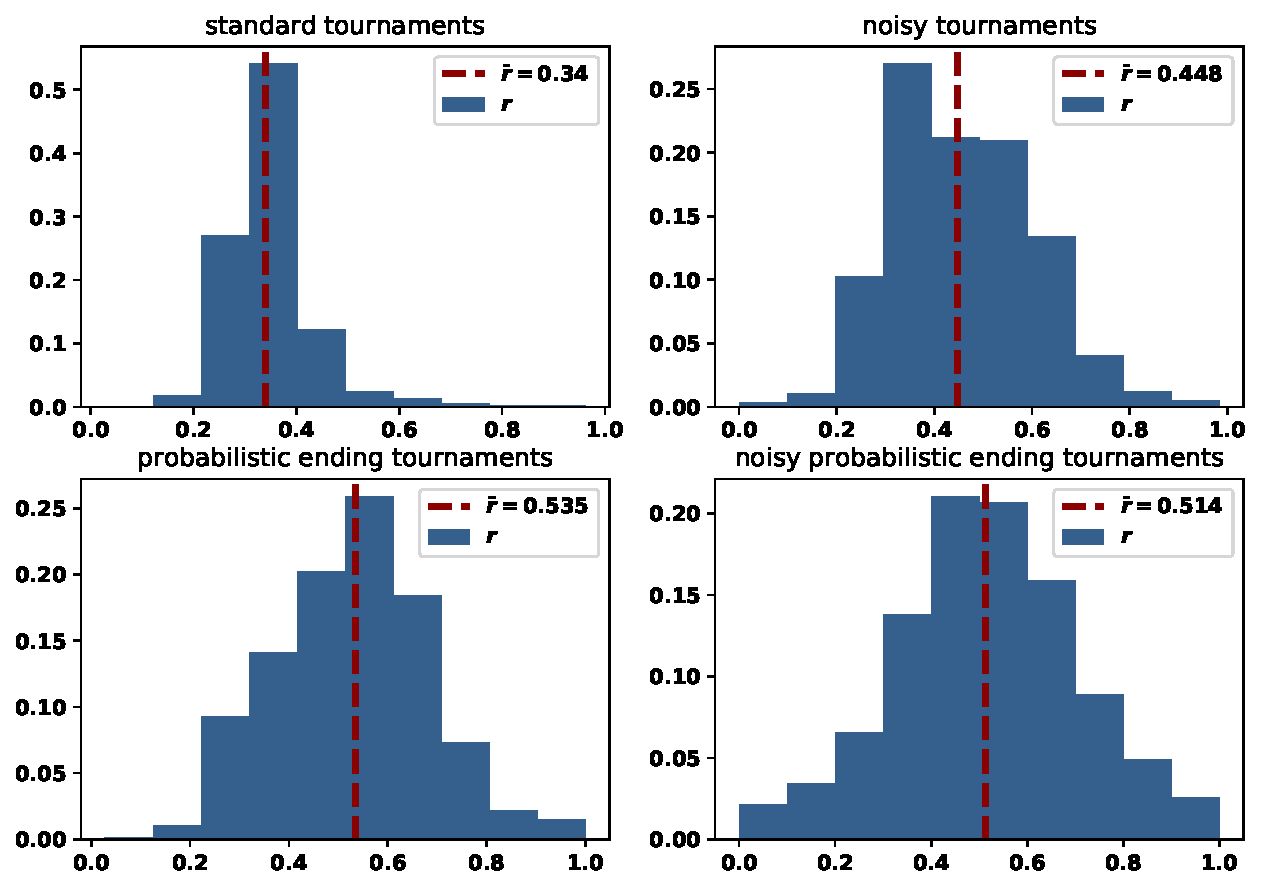
\includegraphics[width=.55\textwidth]{../images/tit_for_tat_r_distributions.pdf}
    \caption{Tit For Tat's $r$ distribution in tournaments. The best performance
    of the strategy has been in standard tournaments where it achieved a $\bar{r}$
    of 0.339.}
    \label{fig:tit_for_tat_r_distribution}
\end{figure}

The top 15 strategies for each tournament type based on \(\bar{r}\) are given in
Table~\ref{table:top_performances}.

\newcolumntype{g}{>{\columncolor{Gray}}l}
\begin{table}[!htbp]
    \begin{center}
    \resizebox{.9\textwidth}{!}{
        \begin{tabular}{lggllggllr}
\toprule
& \multicolumn{2}{g}{Standard} & \multicolumn{2}{c}{Noisy} & \multicolumn{2}{g}{Probabilistic ending} &  \multicolumn{2}{c}{Noisy probabilistic ending} \\
\midrule
& Name & $\bar{r}$ &                 Name & $\bar{r}$ &               Name & $\bar{r}$ &                 Name & $\bar{r}$ \\
\midrule
1 &           Evolved HMM 5 &   0.00667 &               Grumpy &    0.1402 &          Fortress4 &   0.01266 &           Alternator &    0.3037 \\
2 &          Evolved FSM 16 &   0.00995 &                  $e$ &   0.19388 &           Defector &   0.01429 &               $\phi$ &   0.30978 \\
3 &    EvolvedLookerUp2 2 2 &   0.01064 &       Tit For 2 Tats &    0.2069 &  Better and Better &   0.01587 &                  $e$ &    0.3125 \\
4 & Evolved FSM 16 Noise 05 &   0.01667 &         Cycle Hunter &   0.21538 &    Tricky Defector &   0.01875 &                $\pi$ &   0.31686 \\
5 &       PSO Gambler 2 2 2 &   0.02143 &       Risky QLearner &   0.22222 &          Fortress3 &   0.02174 &    Limited Retaliate &   0.35263 \\
6 &             Evolved ANN &   0.02878 &          Retaliate 3 &   0.22887 &     Gradual Killer &   0.02532 &     Anti Tit For Tat &   0.35431 \\
7 &           Evolved ANN 5 &    0.0339 &        Cycler CCCCCD &   0.23507 &         Aggravater &   0.02778 &          Retaliate 3 &   0.35563 \\
8 &       PSO Gambler 1 1 1 &   0.03704 &          Retaliate 2 &   0.23913 &             Raider &   0.03077 &  Limited Retaliate 3 &   0.35563 \\
9 &           Evolved FSM 4 &   0.04891 &      Defector Hunter &   0.24038 &         Cycler DDC &   0.04545 &            Retaliate &   0.35714 \\
10 &        PSO Gambler Mem1 &   0.05036 &            Retaliate &   0.24177 &        Hard Prober &   0.05128 &          Retaliate 2 &   0.35767 \\
11 &                Winner12 &   0.06011 &  Hard Tit For 2 Tats &      0.25 &         SolutionB1 &   0.06024 &  Limited Retaliate 2 &   0.36134 \\
12 &            Fool Me Once &    0.0614 &             ShortMem &   0.25286 &      Meta Minority &   0.06077 &             Hopeless &   0.36842 \\
13 &                     DBS &   0.07143 &  Limited Retaliate 3 &   0.25316 &              Bully &   0.06081 &    Arrogant QLearner &   0.40651 \\
14 &           DoubleCrosser &     0.072 &    Limited Retaliate &   0.25706 &    Fool Me Forever &    0.0708 &    Cautious QLearner &   0.40909 \\
15 &             BackStabber &   0.07519 &                $\pi$ &   0.25801 &             EasyGo &   0.07101 &      Fool Me Forever &   0.41764 \\
\bottomrule
    \end{tabular}
    
    }
\end{center}
\caption{Top performances for each tournament type based on $\bar{r}$.}
\label{table:top_performances}
\end{table}

In standard tournaments 10 out of the 15 top strategies are introduced
in~\cite{Harper2017}. These are strategies based on finite state automata (FSM),
hidden markov models (HMM), artificial neural networks (ANN), lookup tables
(LookerUp) and stochastic lookup tables (Gambler) that have been trained using
reinforcement learning algorithms (evolutionary and particle swarm algorithms).
They have been trained to perform well against the strategies
in~\cite{axelrodproject} in a standard setting, thus their performance in the
specific setting was anticipated. DoubleCrosser, and Fool Me Once, are
strategies not from the literature but from~\cite{axelrodproject}. DoubleCrosser
is a strategy that makes use of the number of turns because is set to defect on
the last two rounds. The strategy was expected to not perform as well in
tournaments where the number of turns is not specified, but the strategy did not
perform well in tournaments with noise either. Finally, Winner
12~\cite{mathieu2017} and DBS~\cite{Au2006} are both from the the literature.
DBS is strategy specifically designed for noisy environments, however, it ranks
highly only in standard ones.

Figure~\ref{fig:std_results} gives the distributions of $r$ for the top
ranked strategies. The distributions are skewed towards zero and the highest
median is at 0.075. This indicates that the top ranked strategies are very
likely to perform well in a standard tournament despite the tournament size,
the opponents, the turns etc.

\begin{figure}[!htbp]
    \centering
    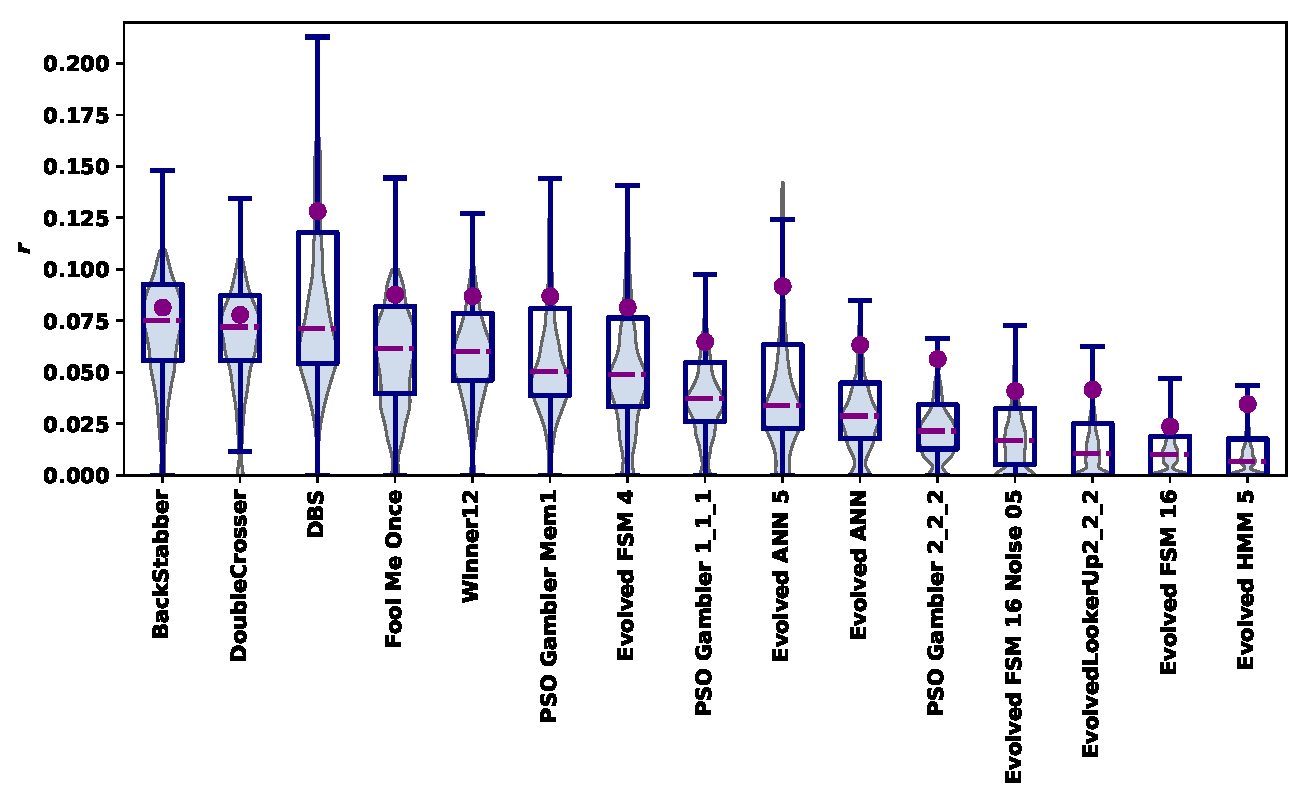
\includegraphics[width=.55\textwidth]{../images/performance_standard.pdf}
    \caption{$r$ distributions of top 15 strategies in standard tournaments.}\label{fig:std_results}
\end{figure}

The top strategies in noisy tournaments are shown in Figure~\ref{fig:noisy_results}. These include deterministic strategies, such
as Tit For 2 Tats~\cite{Axelrod1980b}, Hard Tit For 2 Tats~\cite{Stewart2012}
and Cycler CCCCCD, and strategies which decide their actions based on the
cooperations to defections ratio, such as ShortMem~\cite{Carvalho2013}, Grumpy,
$e$, $\pi$ and $\phi$ (all from~\cite{axelrodproject}). The Retaliate and
Limited Retaliate strategies are implemented in~\cite{axelrodproject} by the
same contributor. The strategies are designed to defect if the opponent has
tricked the strategy more often than \(x\%\) of the times that the strategy has
done the same. Finally, in $4^{\text{th}}$ and $9^{\text{th}}$ are Hunter
strategies which trying to extort, equivalently, strategies that play cyclically
and defectors.

From Figure~\ref{fig:noisy_results}, it is evident that the normalised rank
distributions in noisy environments are more variant with higher medians
compared to standard tournaments. The distributions are bimodal.
This indicates that although the top ranked strategies mainly performed
well, there are several tournaments that they ranked in the bottom half.

\begin{figure}[!htbp]
    \centering
    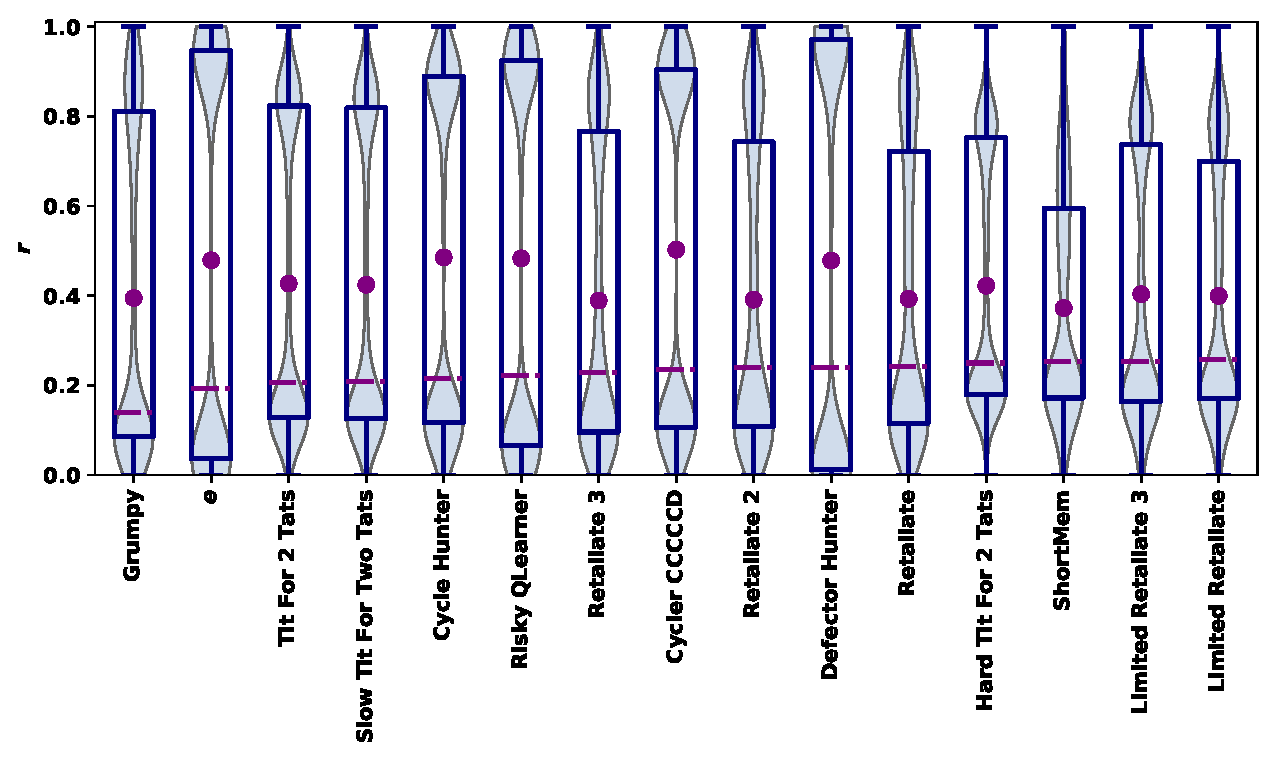
\includegraphics[width=.55\textwidth]{../images/performance_noise.pdf}
    \caption{\(r\) distributions for best performed strategies in noisy tournaments.}
    \label{fig:noisy_results}
\end{figure}

The 15 top ranked strategies in probabilistic ending tournaments include
Fortress 3, Fortress 4 (both introduced in~\cite{Ashlock2006}),
Raider~\cite{Ashlock2014} and Solution B1~\cite{Ashlock2014}, which are
strategies based on finite state automata introduced by Daniel and Wendy
Ashlock. These strategies have been evolved using reinforcement learning, however,
there were trained to maximise their payoffs in tournaments with fixed turns
(150 specifically) and not in probabilistic ending ones. In probabilistic ending
tournaments it appears that the top ranks are mostly occupied by defecting
strategies. These include Better and Better, Gradual Killer, Hard Prober (all
from ~\cite{prison}), Bully (Reverse Tit For Tat)~\cite{Nachbar1992} and
Defector. Thus, it's surprisingly that EasyGo and Fool Me Forever are ranked
$14^{\text{th}}$ and $15^{\text{th}}$. These strategies are actually the same;
they will defect until their opponent defect, then they will cooperate until the
end. Both strategies have repeatedly ranked highly as shown in
Figure~\ref{fig:probend_results}, and there are cases for which they were the
winners of the tournament.

\begin{figure}[h!]
    \centering
    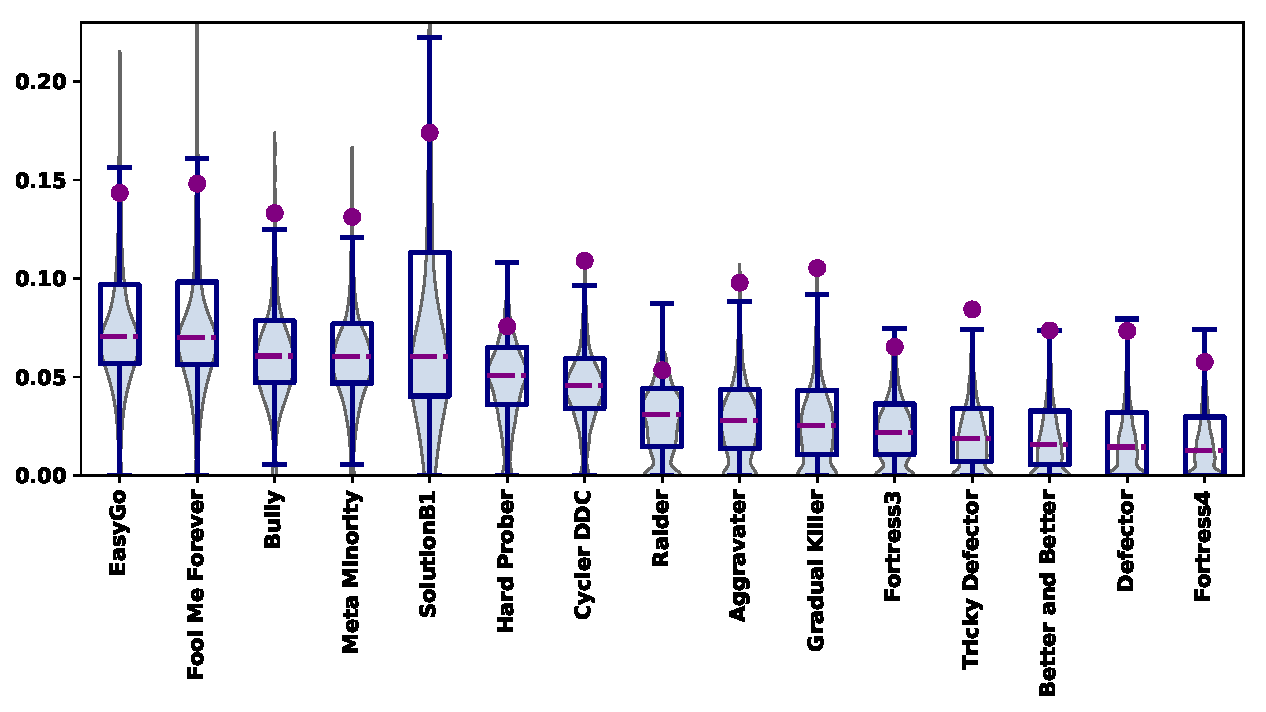
\includegraphics[width=.55\textwidth]{../images/performance_probend.pdf}
    \caption{\(r\) distributions for best performed strategies in probabilistic ending tournaments.}
    \label{fig:probend_results}
\end{figure}

The distributions of the normalised rank in probabilistic ending tournaments,
shown in
Figure~\ref{fig:probend_results}, are less variant than those of noisy
tournaments. The medians are lower than 0.1 and the distributions are skewed
towards 0. Though the large difference between the means and the medians
indicates some outliers, the strategies have overall performed well in the
probabilistic ending tournaments that they participated.

In tournaments with both noise and an unspecified number of turns several of
the top ranked strategies are strategies that were highly ranked in noisy
tournaments. This demonstrates that, $e$, $\pi$,
$\phi$ and the Retaliate family are robust in noisy environments regardless of the
number of turns. However, strategies from the top ranks in probabilistic
ending tournaments did not rank highly here.

\begin{figure}[!htbp]
    \centering
    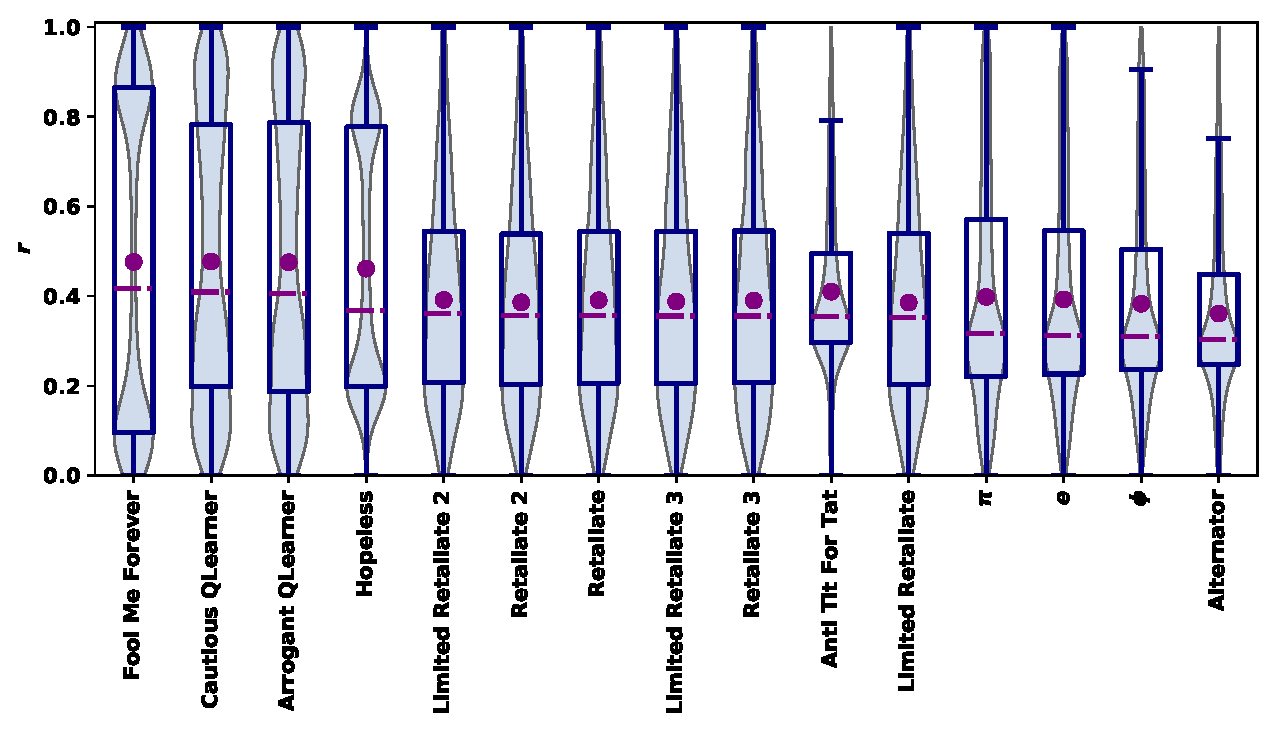
\includegraphics[width=.55\textwidth]{../images/performance_probend_noise.pdf}
    \caption{\(r\) distributions for best performed strategies in noisy
    probabilistic ending tournaments.}
    \label{fig:noisy_probend_results}
\end{figure}

Up till now, the performances of the 194 strategies have been evaluated for
individual tournament types. The data set considered in this work, described in
Section~\ref{section:data_collection}, contains a total of \numberofalltournaments
tournament results. For this part of the manuscript the strategies are ranked
based on the median normalised rank they achieved over the entire data set.
The top 15 strategies are given in Table~\ref{table:overall_results}
and their normalised rank distributions are given in Figure~\ref{fig:overall_results}.

\begin{table}[!htbp]
    \centering
    \resizebox{.35\textwidth}{!}{
    \begin{tabular}{lr}
\toprule
{} &  Normalized\_Rank \\
Name                    &                  \\
\midrule
Evolved FSM 16          &            0.018 \\
Evolved HMM 5           &            0.019 \\
Evolved FSM 16 Noise 05 &            0.025 \\
EvolvedLookerUp2\_2\_2    &            0.028 \\
Evolved ANN             &            0.037 \\
PSO Gambler 2\_2\_2       &            0.040 \\
Evolved ANN 5           &            0.046 \\
PSO Gambler 1\_1\_1       &            0.061 \\
Fool Me Once            &            0.067 \\
Evolved FSM 4           &            0.075 \\
DoubleCrosser           &            0.079 \\
Winner12                &            0.081 \\
BackStabber             &            0.082 \\
DBS                     &            0.086 \\
PSO Gambler Mem1        &            0.089 \\
\bottomrule
\end{tabular}
}
    \caption{Top performances over all the tournaments}\label{table:overall_results}
\end{table}

The top ranks include strategies that have been previously mentioned. The top ranks
are overtaken by the set of Retaliate strategies followed by BackStabber and
DoubleCrosser. DoubleCrosser performed well in standard tournaments and the
strategy is just an extension of BackStabber. PSO Gambler and Evolved HMM 5 are
trained strategies introduced in~\cite{Harper2017} and Nice Meta Winner and NMWE
Memory One are strategies based on teams. Grudger is a strategy from Axelrod's
original tournament and Forgetful Fool Me Once is based on the same approach as
Grudger.

Figure~\ref{fig:overall_results} gives the normalised rank distributions of
these strategies. The distributions of the Retaliate strategies have no
statistical difference. Thus, in an IPD tournament where the type is not
specified, playing as any of the Retaliate strategies will have the result.

\begin{figure}[!htbp]
    \centering
    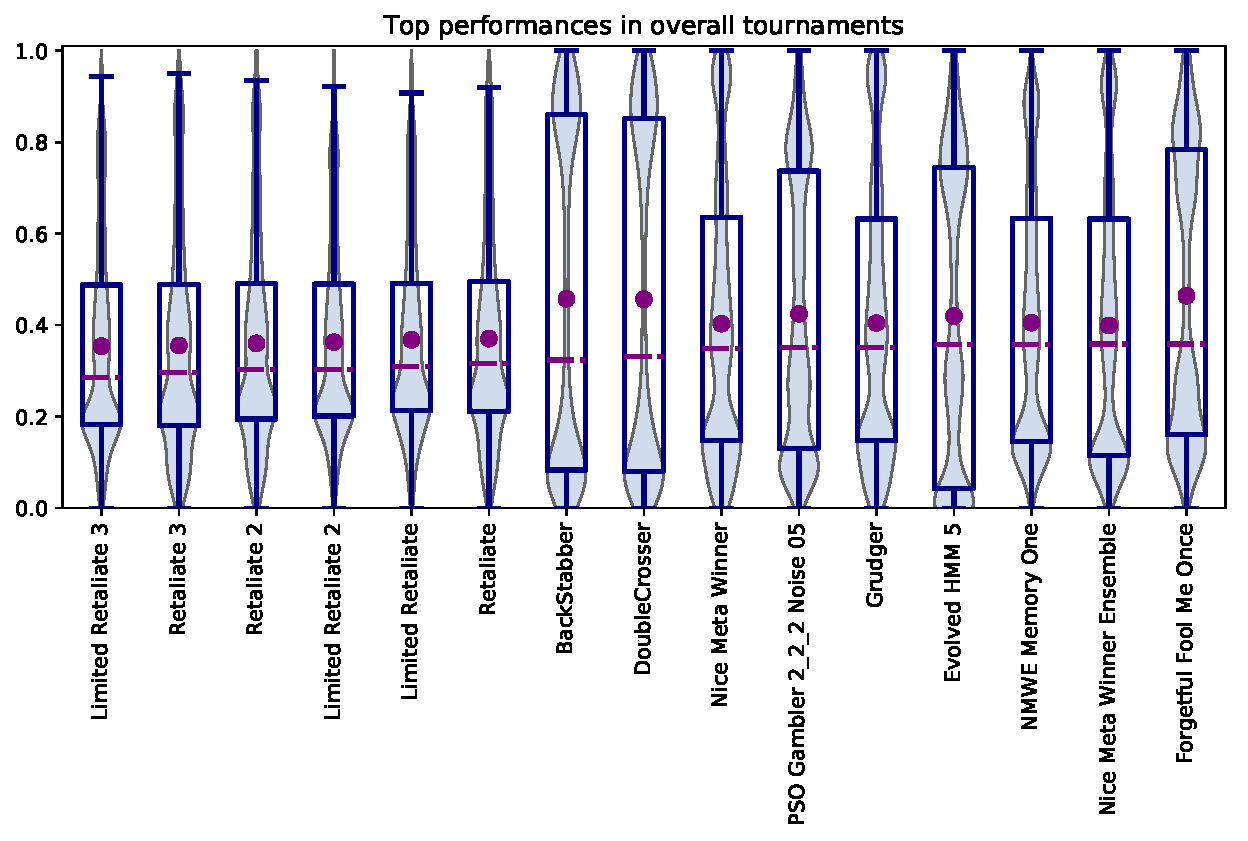
\includegraphics[width=.55\textwidth]{../images/performance_merged.pdf}
    \caption{\(r\) distributions for best performed strategies in the data set~\cite{data}.}
    \label{fig:overall_results}
\end{figure}

This section presented the winning strategies in a series of IPD tournaments. In
standard tournaments the top spots were dominated by complex strategies that had
been trained using reinforcement learning techniques. In noisy environments,
whether the number of turns was fixed or not, the winning strategies were
deterministic strategies designed to defect if the opponent tricked them more
than a current amount of the times that they had tricked their opponent. In
probabilistic ending tournaments most of the winning strategies were defecting
strategies. A few trained finite state automata, designed by the same authors,
also performed well in this setting. Finally the performance of all 194
strategies over the \numberofalltournaments tournaments in this manuscript was
assessed on \(\bar{r}\). The top ranked strategies were a mixture of behaviours
that did well in standard tournaments and tournaments with noise, as well as a
few strategies based on teams.

The results of this section imply that successful strategies for specific
settings exist for an IPD tournament. The top ranked strategies in both standard
tournaments and tournaments with probabilistic ending, managed to rank in the
top 10\% of the tournament most of the times. Strategies successful in noisy
environments demonstrated that they were not affected by the number of turns.
However, there has been not a single strategy that has shown to perform well in
more than one setting. The aim of the next section is to understand which are
the factors that made these strategies successful. In each setting separately
but also overall.

\section{Evaluation of performance}\label{section:evaluation_of_performance}

The aim of this section is to explore the factors that contribute to a
strategy's successful performance. The factors explored are measures regarding a
strategy's behaviour, alogn with measures regarding the tournaments the
strategies competed in. These are given in Table~\ref{table:manual_measures}.

\newcolumntype{g}{>{\columncolor{Gray}}c}
\begin{table}[h]
    \begin{center}
    \resizebox{\textwidth}{!}{
    \begin{tabular}{gcgcgc}
    \toprule
    measure & measure explanation &  source & value type & min value & max value \\
    \midrule
stochastic  &  If a strategy is stochastic & strategy classifier from~\cite{axelrodproject} & boolean  & False &  True \\
makes use of game &  If a strategy makes used of the game information & strategy classifier from~\cite{axelrodproject} & boolean  & False &  True \\
makes use of length &  If a strategy makes used of the number of turns & strategy classifier from~\cite{axelrodproject} & boolean  & False &  True \\
memory usage &  The memory size of a strategy divided by the number of turns & memory size from~\cite{axelrodproject} & float & 0 &  1 \\
SSE & A measure of how far a strategy is from ZD behaviour & method described in~\cite{Knight2019} & float & 0 & 1 \\
max cooperating rate $(C_{\text{max}})$  & The biggest cooperating rate in the tournament  & result summary  & float & 0 & 1\\
min cooperating rate $(C_{\text{min}})$ & The smallest cooperating rate in the tournament  & result summary  & float & 0 & 1\\
median cooperating rate $(C_{\text{median}})$ & The median cooperating rate in the tournament  & result summary  & float & 0 & 1\\
mean cooperating rate $(C_{\text{mean}})$ & The mean cooperating rate in the tournament  & result summary  & float & 0 & 1 \\
$C_r$ / $C_{\text{max}}$ & A strategy's cooperating rate divided by the maximum & result summary  & float & 0 & 1 \\
$C_r$ / $C_{\text{min}}$ & A strategy's cooperating rate divided by the minimum & result summary  & float & 0 & 1 \\
$C_r$ / $C_{\text{median}}$ & A strategy's cooperating rate divided by the median  & result summary  & float & 0 & 1\\
$C_r$ / $C_{\text{mean}}$ & A strategy's cooperating rate divided by the mean & result summary  & float & 0 & 1 \\
$C_r$ & The cooperating ratio of a strategy & result summary  & float & 0 & 1 \\
$CC$ to $C$ rate & The probability a strategy will cooperate after a mutual cooperation & result summary  & float & 0 & 1\\
$CD$ to $C$ rate & The probability a strategy will cooperate after being betrayed by the opponent & result summary  & float & 0 & 1 \\
$DC$ to $C$ rate & The probability a strategy will cooperate after betraying the opponent & result summary  & float & 0 & 1 \\
$DD$ to $C$ rate & The probability a strategy will cooperate after a mutual defection & result summary  & float & 0 & 1 \\
$p_n$ & The probability of a player's action being flip at each interaction & trial summary & float & 0 & 1 \\
$n$ & The number of turns & trial summary & integer & 1 & 200 \\
$p_e$ & The probability of a match ending in the next turn & trial summary & float & 0 & 1 \\
$N$ & The number of strategies in the tournament & trial summary & integer & 3 & 195 \\
$k$ & The number of repetitions of a given tournament & trial summary & integer & 10 & 100 \\
    \bottomrule
        \end{tabular}}
    \end{center}
    \caption{The measures which are included in the performance evaluation analysis.}
    \label{table:manual_measures}
\end{table}

Axelrod-Python makes use of classifiers to classify strategies according to
various dimensions. These determine whether
a strategy is stochastic or deterministic, whether it makes use of the number of
turns or the game's payoffs. The memory usage measure is calculated as the
memory size of strategy (which is specified in the strategies implementation
in~\cite{axelrodproject}) divide by the number of turns. For tournaments with a
probabilistic ending the number of turns has been not collected, so the memory
usage measure is not used for probabilistic ending tournaments.
The SSE is a measure of extortionate behaviour introduced in~\cite{Knight2019}.
A value of 1 indicates no extortionate behaviour at all whereas a value of 0
indicates that a strategy is always trying to extortion it's opponent. The rest
of the factors considered are the $CC$ to $C$, $CD$ to $C$, $DC$ to $C$, and
$DD$ to $C$ rates as well as cooperating ratio of a strategy. The minimum,
maximum, medium and median cooperating ratios of each tournament are also
included, and finally the number of turns, the number of strategies and the
probabilities of noise and the game ending are also included.

Table~\ref{table:correlations} shows the correlation coefficients between the
measures of Table~\ref{table:manual_measures} the median score and the median
normalised rank. Note that the correlation for the classifiers is
not included because they are binary variables and they will be evaluated using a
different method. The correlation coefficients for all the measures in
Table~\ref{table:manual_measures} against themselves have also been calculated and a
graphical representation can be found in the Appendix~\ref{app:correlations}.

\newcolumntype{g}{>{\columncolor{Gray}}c}
\begin{table}[!htbp]
    \begin{center}
    \resizebox{.9\textwidth}{!}{
        \begin{tabular}{lggccggccggg}
    \toprule
    &  \multicolumn{2}{g}{Standard} & \multicolumn{2}{c}{Noisy} & \multicolumn{2}{g}{Probabilistic ending} &  \multicolumn{2}{c}{Noisy probabilistic ending} &  \multicolumn{2}{g}{Overall} \\
\midrule
{} &  $r$ &  median score &  $r$ &  median score &  $r$ &  median score &  $r$ &  median score &  $r$ &  median score\\
\midrule
$CC$ to $C$ rate     & -0.501 &  0.501 &   0.414 &  -0.504 &   0.408 &  -0.323 &   0.260 &   0.022 &  -0.501 &  0.501 \\
$CD$ to $C$ rate     &  0.226 & -0.199 &   0.456 &  -0.330 &   0.320 &  -0.017 &   0.205 &  -0.220 &   0.226 & -0.199 \\
$C_r$                & -0.323 &  0.384 &   0.711 &  -0.678 &   0.714 &  -0.832 &   0.579 &  -0.135 &  -0.323 &  0.384 \\
$C_r$ / $C_{max}$    & -0.323 &  0.381 &   0.616 &  -0.551 &   0.714 &  -0.833 &   0.536 &  -0.116 &  -0.323 &  0.381 \\
$C_r$ / $C_{mean}$   & -0.331 &  0.358 &   0.731 &  -0.740 &   0.721 &  -0.861 &   0.649 &  -0.621 &  -0.331 &  0.358 \\
$C_r$ / $C_{median}$ & -0.331 &  0.353 &   0.652 &  -0.669 &   0.712 &  -0.852 &   0.330 &  -0.466 &  -0.331 &  0.353 \\
$C_r$ / $C_{min}$    &  0.109 & -0.080 &  -0.358 &   0.250 &  -0.134 &   0.150 &  -0.368 &   0.113 &   0.109 & -0.080 \\
$C_{max}$            & -0.000 &  0.049 &   0.000 &   0.023 &  -0.000 &   0.046 &   0.000 &  -0.004 &  -0.000 &  0.049 \\
$C_{mean}$           & -0.000 &  0.229 &  -0.000 &   0.271 &   0.000 &   0.200 &   0.000 &   0.690 &  -0.000 &  0.229 \\
$C_{median}$         &  0.000 &  0.209 &  -0.000 &   0.240 &  -0.000 &   0.187 &  -0.000 &   0.673 &   0.000 &  0.209 \\
$C_{min}$            &  0.000 &  0.084 &   0.000 &  -0.017 &  -0.000 &   0.007 &  -0.000 &   0.041 &   0.000 &  0.084 \\
$DC$ to $C$ rate     &  0.127 & -0.100 &   0.509 &  -0.504 &  -0.018 &   0.033 &   0.341 &  -0.016 &   0.127 & -0.100 \\
$DD$ to $C$ rate     &  0.412 & -0.396 &   0.533 &  -0.436 &  -0.103 &   0.176 &   0.378 &  -0.263 &   0.412 & -0.396 \\
$N$                  &  0.000 & -0.009 &  -0.000 &   0.002 &  -0.000 &   0.003 &  -0.000 &   0.001 &   0.000 & -0.009 \\
$k$                  &  0.000 & -0.002 &  -0.000 &   0.003 &  -0.000 &   0.001 &  -0.000 &  -0.008 &   0.000 & -0.002 \\
$n$                  &  0.000 & -0.125 &  -0.000 &  -0.024 &       - &       - &       - &       - &   0.000 & -0.125 \\
$p_e$                &      - &      - &        - &     - &    0.000 &   0.165 &   0.000 &  -0.058 &  -0.001 &  0.001 \\
$p_n$                &      - &      - &  -0.000 &   0.207 &       - &       - &  -0.000 &  -0.650 &   0.002 & -0.000 \\
Make use of game     & -0.003 & -0.022 &   0.025 &  -0.082 &  -0.053 &  -0.108 &   0.013 &  -0.016 &  -0.003 & -0.022 \\
Make use of length   & -0.158 &  0.124 &   0.005 &  -0.123 &  -0.025 &  -0.090 &   0.014 &  -0.016 &  -0.154 &  0.117 \\
SSE                  &  0.473 & -0.452 &   0.463 &  -0.337 &  -0.156 &   0.223 &   0.305 &  -0.259 &   0.473 & -0.452 \\
memory usage         & -0.082 &  0.095 &  -0.007 &  -0.017 &       - &     - &     - &           - &  -0.084 &  0.095 \\
stochastic           &  0.006 & -0.024 &   0.022 &  -0.026 &   0.002 &  -0.130 &   0.021 &  -0.013 &   0.006 & -0.024 \\
\bottomrule
\end{tabular}

    }
\end{center}
\caption{Correlations table between the measures of Table~\ref{table:manual_measures}
the normalised rank and the median score.}\label{table:correlations}
\end{table}

In standard tournaments the measures  $CC$ to $C$, $C_r$, $C_r / C_{\text{max}}$
and the cooperating ratio compared to $C_{\text{median}}$ and $C_{\text{mean}}$
have a moderate negative effect on the normalised rank, and a moderate positive
on the median score. The SSE error and the $DD$ to $C$ have the opposite
effects. Thus, in standard tournaments behaving cooperatively corresponds to a
more successful performance. Even though being nice pays off,
that's not true against defective strategies. Cooperating after a mutual
defection lowers a strategy's success.
Figure~\ref{fig:rates_of_winners_in_standard_tournaments} confirms that the
winners of standard tournaments always cooperate after a mutual cooperation and
almost always defects after a mutual defection.

\begin{figure}[!htbp]
    \centering
    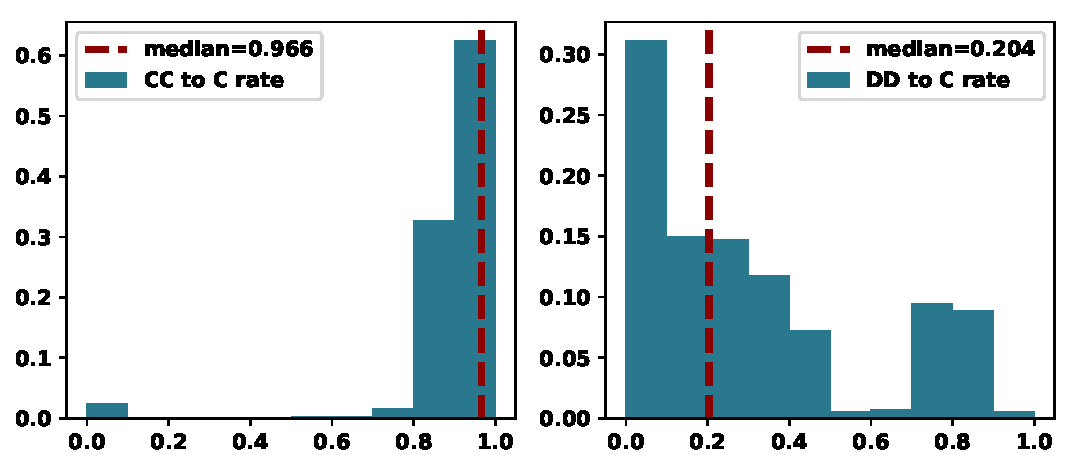
\includegraphics[width=.5\textwidth]{../images/rates_of_winners_in_standard_tournaments.pdf}
    \caption{Distributions of $CC$ to $C$ and $DD$ to $C$ for the winners in
    standard tournaments.}\label{fig:rates_of_winners_in_standard_tournaments}
\end{figure}

Compared to standard tournaments, in both noisy and in probabilistic ending
tournaments the higher the rates of cooperation the lower a strategy's success
and median score. A strategy would want to cooperate less than both
the mean and median cooperator in such settings. In probabilistic ending
tournaments the correlations coefficients have a larger values, indicating a
stronger effect. Thus a strategy will be punished more by it's cooperative
behaviour in probabilistic ending environments. The distributions of the $C_r$ of the winners in
both tournaments is given by Figure~\ref{fig:c_r_distributions}. It confirms
that the winners in noisy tournaments cooperated less than 35\% of the times
and in probabilistic ending tournaments less than 10\%.

\begin{figure}[!htbp]
    \centering
    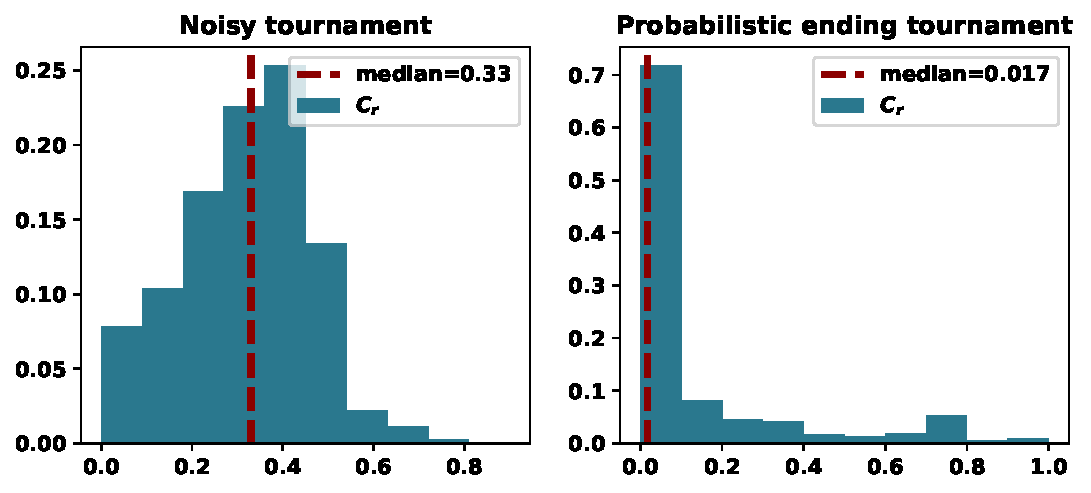
\includegraphics[width=.5\textwidth]{../images/c_r_winners_tournaments.pdf}
    \caption{$C_r$ distributions of the winners in noisy and in probabilistic
    ending tournaments.}\label{fig:c_r_distributions}
\end{figure}

In noisy probabilistic ending tournaments and in over all the tournaments' results,
the only measures that had a moderate affect are $C_r/C_{\text{mean}},
C_r/C_{\text{max}}$ and $C_r$. In such environments cooperative behaviour
appears to be punished by not as much as in noisy and probabilistic ending
tournaments.

The effect of the measures on performances is further tested using a random forest
classification~\cite{breiman2001} approach. Initially, the performances are
clustered based on their normalised rank and the median score by a \(k-\)means
algorithm~\cite{Arthur2007}. The number of clusters is not deterministically
chosen but it is based on the silhouette coefficients~\cite{Rousseeuw1987}.
Consider the case of standard tournaments, the chosen number of clusters is
2 and Figure~\ref{fig:standard_clusters} illustrates the trials of clustering the
performances in 2, 3 and 4 clusters respectively. The number of chosen clusters
for each type and overall are given in Table~\ref{table:number_of_clusters}.

\begin{figure}[!htbp]
\centering
\includegraphics[width=.55\textwidth]{../output/standard/clusters_plots.png}
\caption{Clustering trials for standard tournaments. A number of 2 clusters has
been chosen with a silhouette score of  0.66 against 0.511 and 0.50
respectively.}\label{fig:standard_clusters}
\end{figure}

\begin{table}[!htbp]
    \begin{center}
        \resizebox{.5\textwidth}{!}{
        \begin{tabular}{lcccc}
    \toprule
    Tournament type & Number of clusters &  Silhouette coefficient\\
    \midrule
    standard                   & 2 & 0.648 \\
    noisy                      & 3 & 0.493 \\
    probabilistic ending       & 2 & 0.680 \\
    noisy probabilistic ending & 4 & 0.415\\
    over \numberofalltournaments tournaments         & 3 & 0.443\\
    \bottomrule
        \end{tabular}}
    \end{center}
    \caption{Number of clusters for each type and over all the tournament results
    and the respective silhouette coefficients.}
    \label{table:number_of_clusters}
\end{table}

A random forest approach is applied to the data to predict the cluster to which
a strategy's performance has been assigned to. The random forest method
constructs many individual decision trees and the predictions from all trees are
pooled to make the final prediction. The random forest models are trained on a
training set of 70\% of the tournaments results. The accuracy of each model
based on $R^2$ are given by Table~\ref{table:accuracy_random_forest}. The out of
the bag error~\cite{hastie2005} has also been calculated. The models fit well, and
a high value of both the accuracy measure on the test data and the
OOB error indicate that the model is not over fitting.

\begin{table}[!htbp]
    \begin{center}
        \resizebox{.5\textwidth}{!}{
        \begin{tabular}{lcccc}
    \toprule
    Tournament type & $R^2$ training data &  $R^2$ test data  & $R^2$ OOB score\\
    \midrule
    standard                   & 0.998545  & 0.989890 & 0.982331\\
    noisy                      & 0.996677  & 0.950572 & 0.935383\\
    probabilistic ending       & 0.999592  & 0.995128 & 0.992819 \\
    noisy probabilistic ending & 0.990490  & 0.813905 & 0.791418\\
    over \numberofalltournaments tournaments & 0.993396 & 0.913409 & 0.898059 \\
    \bottomrule
        \end{tabular}}
    \end{center}
    \caption{Accuracy metrics for random forest models.}
    \label{table:accuracy_random_forest}
\end{table}

The importance that the measures of Table~\ref{table:manual_measures} had on the
classification task; to which cluster a performance was assigned to, have been
calculated and are given by Figure~\ref{fig:importance}. The classifiers which
where not included in the previous analysis appear to have no effect, and
several of the measures that are highted by the importance are inline with the
correlation results. The most important measures based on the random forest
analysis were $C_r / C_{median}$ and $C_r / C_{mean}$.

\begin{figure}[!htbp]
    \begin{minipage}{0.5\textwidth}
        \begin{center}
            \includegraphics[width=.75\linewidth]{../output/standard/_feature_importance_bar_plot.pdf}
        \end{center}
        \caption{Standard tournaments}
    \end{minipage}\hspace{1cm}
    \begin{minipage}{0.5\textwidth}
        \begin{center}
            \includegraphics[width=.75\linewidth]{../output/noise/_feature_importance_bar_plot.pdf}
        \end{center}
        \caption{Noisy tournaments}
    \end{minipage}\hspace{1cm}
    \begin{minipage}{0.5\textwidth}
        \begin{center}
            \includegraphics[width=.75\linewidth]{../output/probend/_feature_importance_bar_plot.pdf}
        \end{center}
        \caption{Probabilistic ending tournaments}
    \end{minipage}\hspace{1cm}
    \begin{minipage}{0.5\textwidth}
        \begin{center}
            \includegraphics[width=.75\linewidth]{../output/probend_noise/_feature_importance_bar_plot.pdf}
        \end{center}
        \caption{Noisy probabilistic ending tournaments}
    \end{minipage}
    \begin{minipage}{0.5\textwidth}
    \end{minipage}\hspace{4.5cm}
    \begin{minipage}{0.5\textwidth}
        \begin{center}
            \includegraphics[width=.75\linewidth]{../output/merged/_feature_importance_bar_plot.pdf}
        \end{center}
        \caption{overall ending tournaments}
    \end{minipage}
    \caption{Importance of features in IPD tournaments.}\label{fig:importance}
\end{figure}

The effect of both these measures can be further explored. Their distributions
for the winners of the tournaments are given by
Figures~\ref{fig:mean_median_std},~\ref{fig:mean_median_noisy},
\ref{fig:mean_median_probend}, \ref{fig:mean_median_probend_noisy} and
\ref{fig:mean_median_overall}. The results suggest that if a strategy with
a theory of mind competed in a standard tournament, then the strategy would
want to be the mean/median cooperator of that tournament. In comparison, if the
same strategy competed in a tournament with noisy or the strategy had no
information regarding the setting of the tournament, then it would
want to cooperate 67\% of the times the mean or median cooperator did.
In probabilistic ending tournament it has already been mentioned that defecting
strategies prevail. This result is once again confirmed in this section.

\begin{figure}[!htbp]
    \centering
    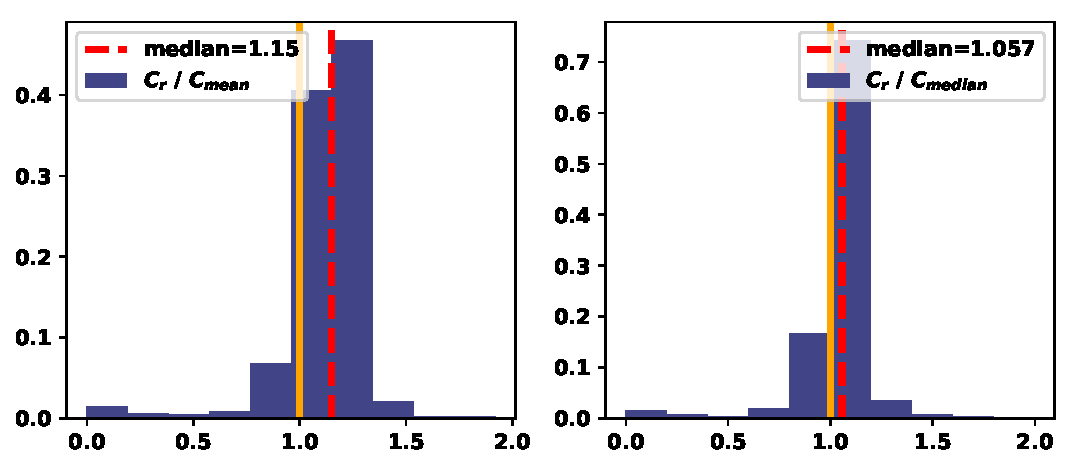
\includegraphics[width=.5\textwidth]{../images/compared_to_mean_median_standard.pdf}
    \caption{Distributions of \(C_r / C_{\text{median}}\)
    and \(C_r / C_{\text{median}}\) for winners of standard tournaments.}\label{fig:mean_median_std}
\end{figure}

\begin{figure}[!htbp]
    \centering
    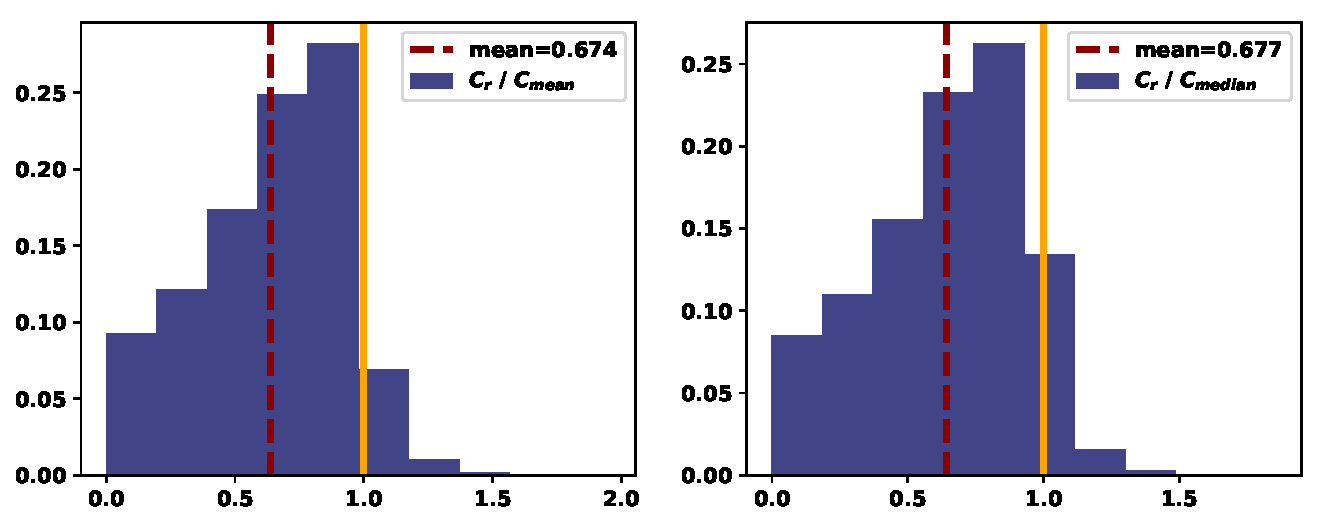
\includegraphics[width=.5\textwidth]{../images/compared_to_mean_median_noisy.pdf}
    \caption{Distributions of \(C_r / C_{\text{median}}\)
    and \(C_r / C_{\text{median}}\) for winners of noisy tournaments.}\label{fig:mean_median_noisy}
\end{figure}

\begin{figure}[!htbp]
    \centering
    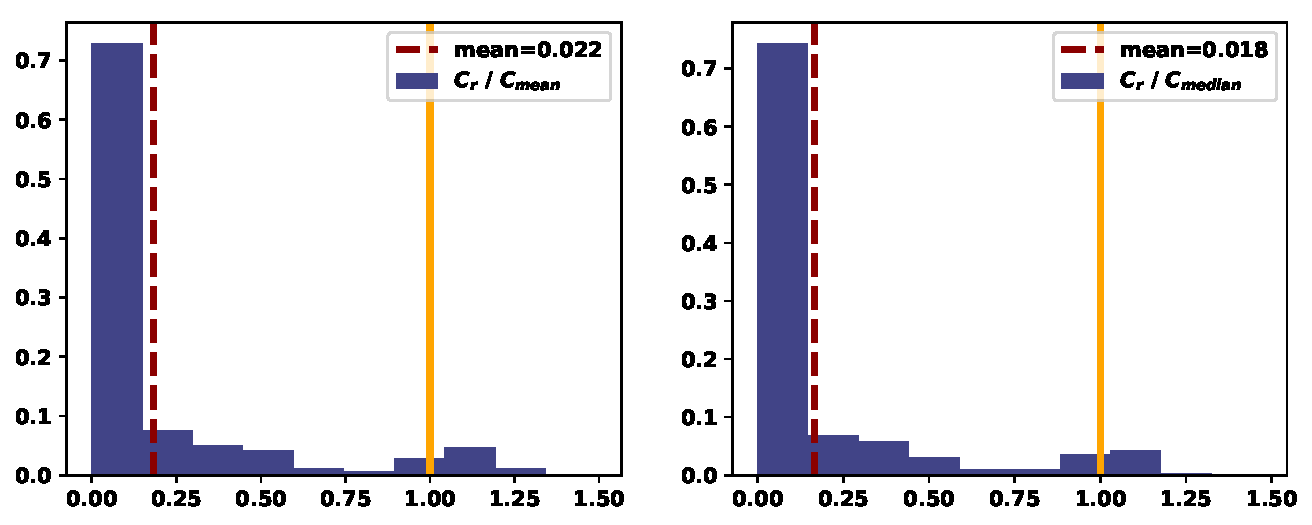
\includegraphics[width=.5\textwidth]{../images/compared_to_mean_median_probend.pdf}
    \caption{Distributions of \(C_r / C_{\text{median}}\)
    and \(C_r / C_{\text{median}}\) for winners of probabilistic ending tournaments.}\label{fig:mean_median_probend}
\end{figure}

\begin{figure}[!htbp]
    \centering
    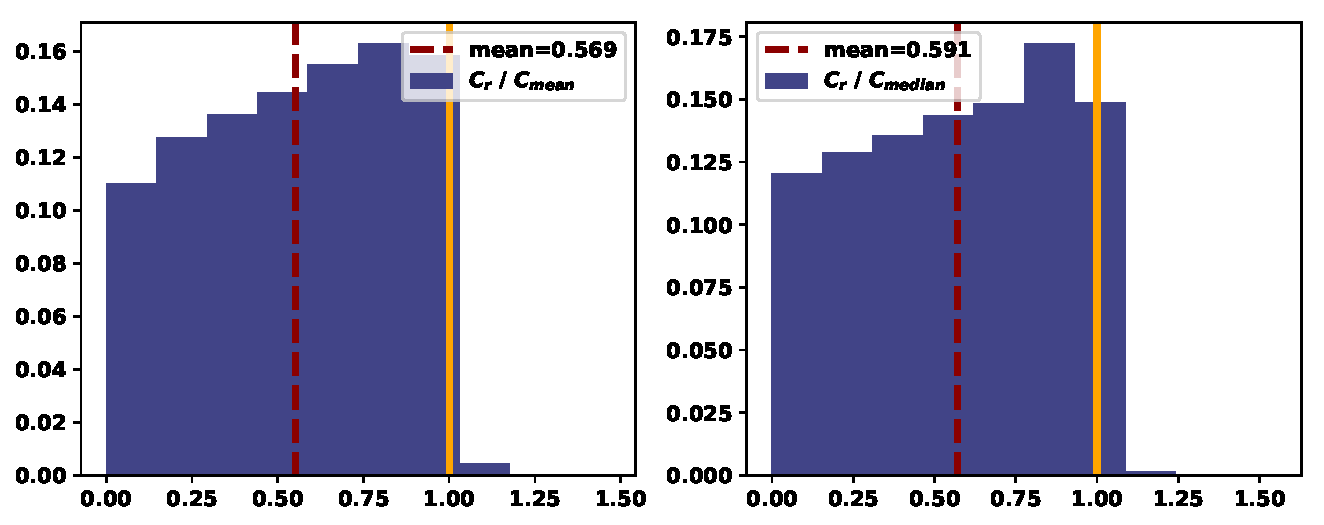
\includegraphics[width=.5\textwidth]{../images/compared_to_mean_median_probend_noisy.pdf}
    \caption{Distributions of \(C_r / C_{\text{median}}\)
    and \(C_r / C_{\text{median}}\) for winners of noisy probabilistic ending tournaments.}\label{fig:mean_median_probend_noisy}
\end{figure}

\begin{figure}[!htbp]
    \centering
    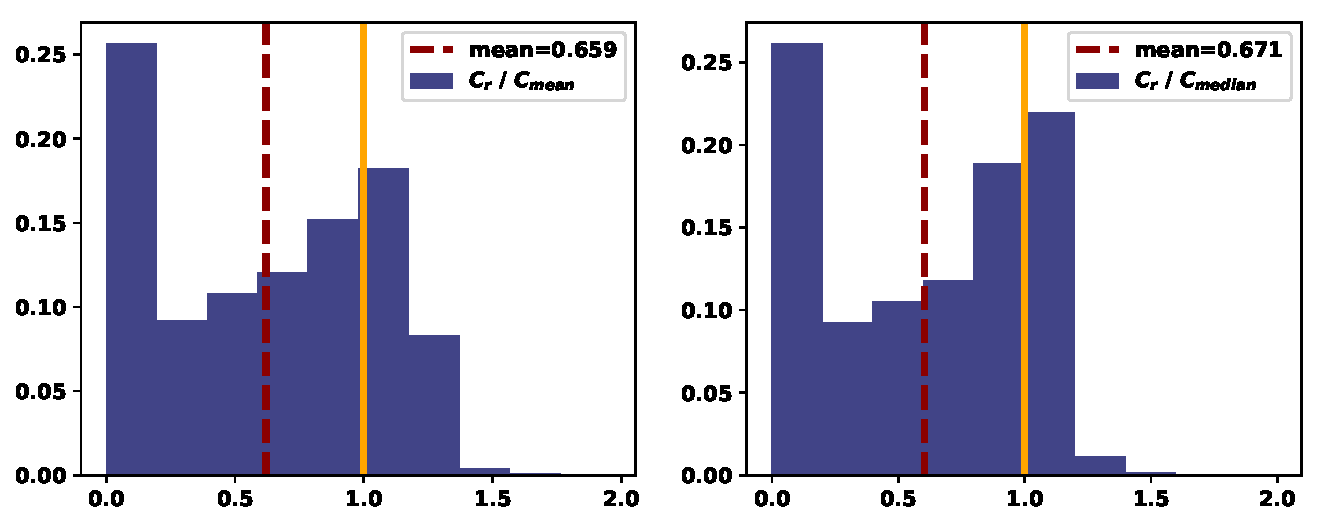
\includegraphics[width=.5\textwidth]{../images/compared_to_mean_median_overall.pdf}
    \caption{Distributions of \(C_r / C_{\text{median}}\)
    and \(C_r / C_{\text{median}}\) for winners of over all the tournaments.}\label{fig:mean_median_overall}
\end{figure}

In this section the effect of several measures, regarding a strategy's behaviour
and the tournament, on it's performance were presented. This was done using
two approaches. Correlation coefficients and a random forest
analysis. The results of these are discussed in the following section.

\section{Conclusion}\label{section:conclusion}

This manuscript has explored the performance of 194 strategies of the Iterated
Prisoner's Dilemma in a large number of computer tournaments. The results of
the analysis demonstrated that, although for specific tournament type, such as
standard, noisy and probabilistic ending tournaments, dominant strategies exist
there is not a single dominant strategy if the environments
vary. Moreover, a strategy with a theory of mind should aim to adapt its behaviour
based on the mean and median cooperators.

The 194 strategies used in this manuscript have been mainly for the literature,
and they have been accessible due to an open source software called
Axelrod-Python. The software was used to generate a total of
\numberofalltournaments computer tournaments results with different number of
strategies and different participants each time. The data collection was
described in Section~\ref{section:data_collection}. In
Section~\ref{section:top_performances}, the tournaments results were used to
present the top performances.
The data set contained results from four different settings, and these were also
studied individually. In standard tournaments complex strategies trained using
reinforcement learning ranked in the top places. In probabilistic ending
tournaments, several trained strategies based on finite state automata also
performed well. The rest top strategies, in this setting, were defecting
strategies. Finally, in tournaments with noise, the Retaliate set of strategies
demonstrated their robustness in tournaments with probabilistic ending and not.

Section~\ref{section:evaluation_of_performance}, covered an analysis of
performance based on several measures associated with a strategy and with the
environments it was competing. The results of this analysis showed that a
strategy's characteristics such as whether or not it's stochastic, and the information it
used regarding the game had no effect on the strategy's success. The most
important factors have been those that compared the strategy's behaviour to it's
environment. The cooperating ratio of the strategy compared to the mean and
median cooperator was highlighted as the most important feature in the analysis.
More specifically, if a strategy were to enter a tournament with a theory of
mind of it's environment it would choose to be the median cooperator in standard
tournaments, the defector in probabilistic ending tournaments and to cooperate
60\% of the times the median cooperator did in noisy and noisy probabilistic
tournaments. Lastly, if a strategy was aware of the opponents but not of the
setting on the tournament, a strategy would be more likely to be successful if
it were to identify the median cooperator and cooperated 67\% of the times that
they did.

\bibliographystyle{plain}
\bibliography{bibliography}

\section{Acknowledgements}

A variety of software have been used in this work:

\begin{itemize}
    \item The Axelrod library for IPD simulations~\cite{axelrodproject}.
    \item The Matplotlib library for visualisation~\cite{hunter2007matplotlib}.
    \item The Numpy library for data manipulation~\cite{walt2011numpy}.
    \item The scikit-learn library for data analysis~\cite{scikit-learn}.
\end{itemize}

\appendix

\section{A summary of parameters}\label{app:parameters}


\begin{table}[h]
    \begin{center}
    \resizebox{.7\textwidth}{!}{
    \begin{tabular}{llc}
    \toprule
measure & measure explanation \\
 \midrule
stochastic                  & If a strategy is stochastic \\
makes use of game           & If a strategy makes used of the game information  \\
makes use of length         & If a strategy makes used of the number of turns \\
memory usage                & The memory size of a strategy divided by the number of turns \\
SSE                         & A measure of how far a strategy is from extortionate behaviour \\
$(C_{\text{max}})$          & The biggest cooperating rate in the tournament \\
$(C_{\text{min}})$          & The smallest cooperating rate in the tournament \\
$(C_{\text{median}})$       & The median cooperating rate in the tournament \\
$(C_{\text{mean}})$         & The mean cooperating rate in the tournament \\
$C_r$ / $C_{\text{max}}$    & A strategy's cooperating rate divided by the maximum \\
$C_r$ / $C_{\text{min}}$    & A strategy's cooperating rate divided by the minimum \\
$C_r$ / $C_{\text{median}}$ & A strategy's cooperating rate divided by the median \\
$C_r$ / $C_{\text{mean}}$   & A strategy's cooperating rate divided by the mean \\
$C_r$                       & The cooperating ratio of a strategy \\
$CC$ to $C$ rate            & The probability a strategy will cooperate after a mutual cooperation \\
$CD$ to $C$ rate            & The probability a strategy will cooperate after being betrayed by the opponent \\
$DC$ to $C$ rate            & The probability a strategy will cooperate after betraying the opponent\\
$DD$ to $C$ rate            & The probability a strategy will cooperate after a mutual defection\\
$p$                         & The probability of a player's action being flip at each interaction \\
$n$                         & The number of turns \\
$e$                         & The probability of a match ending in the next turn \\
$N$                         & The number of strategies in the tournament \\
    \bottomrule
        \end{tabular}}
    \end{center}
    \caption{The measures which are included in the performance evaluation analysis.}
\end{table}



\section{List of strategies}\label{app:list_of_players}

The strategies used in this study which are from Axelrod version 3.0.0
\cite{axelrodproject}.

\begin{multicols}{3}
	\begin{enumerate}
		\item $\phi$~\cite{axelrodproject}
\item $\pi$~\cite{axelrodproject}
\item $e$~\cite{axelrodproject}
\item ALLCorALLD \cite{axelrodproject}
\item Adaptive~\cite{Li2011}
\item Adaptive Pavlov 2006~\cite{kendall2007iterated}
\item Adaptive Pavlov 2011~\cite{Li2011}
\item Adaptive Tit For Tat: 0.5~\cite{Tzafestas2000}
\item Aggravater~\cite{axelrodproject}
\item Alexei~\cite{lesswrong}
\item Alternator~\cite{Axelrod1981, Mittal2009}
\item Alternator Hunter~\cite{axelrodproject}
\item Anti Tit For Tat~\cite{Hilbe2013}
\item AntiCycler~\cite{axelrodproject}
\item Appeaser~\cite{axelrodproject}
\item Arrogant QLearner~\cite{axelrodproject}
\item Average Copier~\cite{axelrodproject}
\item Backstabber~\cite{axelrodproject}
\item Better and Better~\cite{prison}
\item Bully~\cite{Nachbar1992}
\item Calculator~\cite{prison}
\item Cautious QLearner~\cite{axelrodproject}
\item Champion~\cite{Axelrod1980b}
\item CollectiveStrategy~\cite{Li2009}
\item Contrite Tit For Tat~\cite{Axelrod1995}
\item Cooperator~\cite{Axelrod1981, Mittal2009, Press2012}
\item Cooperator Hunter~\cite{axelrodproject}
\item Cycle Hunter~\cite{axelrodproject}
\item Cycler CCCCCD~\cite{axelrodproject}
\item Cycler CCCD~\cite{axelrodproject}
\item Cycler CCCDCD~\cite{axelrodproject}
\item Cycler CCD~\cite{Mittal2009}
\item Cycler DC~\cite{axelrodproject}
\item Cycler DDC~\cite{Mittal2009}
\item DBS~\cite{Au2006}
\item Davis~\cite{Axelrod1980a}
\item Defector~\cite{Axelrod1981, Mittal2009, Press2012}
\item Defector Hunter~\cite{axelrodproject}
\item Double Crosser~\cite{axelrodproject}
\item Desperate \cite{Van2015}
\item DoubleResurrection~\cite{Eckhart2015}
\item Doubler~\cite{prison}
\item Dynamic Two Tits For Tat~\cite{axelrodproject}
\item EasyGo~\cite{Li2011, prison}
\item Eatherley~\cite{Axelrod1980b}
\item Eventual Cycle Hunter~\cite{axelrodproject}
\item Evolved ANN~\cite{axelrodproject}
\item Evolved ANN 5~\cite{axelrodproject}
\item Evolved ANN 5 Noise 05~\cite{axelrodproject}
\item Evolved FSM 16~\cite{axelrodproject}
\item Evolved FSM 16 Noise 05~\cite{axelrodproject}
\item Evolved FSM 4~\cite{axelrodproject}
\item Evolved HMM 5~\cite{axelrodproject}
\item EvolvedLookerUp1 1 1~\cite{axelrodproject}
\item EvolvedLookerUp2 2 2~\cite{axelrodproject}
\item Eugine Nier~\cite{lesswrong}
\item Feld~\cite{Axelrod1980a}
\item Firm But Fair~\cite{Frean1994}
\item Fool Me Forever~\cite{axelrodproject}
\item Fool Me Once~\cite{axelrodproject}
\item Forgetful Fool Me Once~\cite{axelrodproject}
\item Forgetful Grudger~\cite{axelrodproject}
\item Forgiver~\cite{axelrodproject}
\item Forgiving Tit For Tat~\cite{axelrodproject}
\item Fortress3~\cite{Ashlock2006}
\item Fortress4~\cite{Ashlock2006}
\item GTFT \cite{Gaudesi2016, Nowak1993}
\item General Soft Grudger~\cite{axelrodproject}
\item Gradual~\cite{Beaufils1997}
\item Gradual Killer~\cite{prison}
\item Grofman\cite{Axelrod1980a}
\item Grudger~\cite{Axelrod1980a, Banks1990, Beaufils1997, Van2015, Li2011}
\item GrudgerAlternator~\cite{prison}
\item Grumpy~\cite{axelrodproject}
\item Handshake~\cite{Robson1990}
\item Hard Go By Majority~\cite{Mittal2009}
\item Hard Go By Majority: 10~\cite{axelrodproject}
\item Hard Go By Majority: 20~\cite{axelrodproject}
\item Hard Go By Majority: 40~\cite{axelrodproject}
\item Hard Go By Majority: 5~\cite{axelrodproject}
\item Hard Prober~\cite{prison}
\item Hard Tit For 2 Tats~\cite{Stewart2012}
\item Hard Tit For Tat~\cite{PD2017}
\item Hesitant QLearner\cite{axelrodproject}
\item Hopeless~\cite{Van2015}
\item Inverse~\cite{axelrodproject}
\item Inverse Punisher~\cite{axelrodproject}
\item Joss~\cite{Axelrod1980a, Stewart2012}
\item Knowledgeable Worse and Worse~\cite{axelrodproject}
\item Level Punisher~\cite{Eckhart2015}
\item Limited Retaliate 2~\cite{axelrodproject}
\item Limited Retaliate 3~\cite{axelrodproject}
\item Limited Retaliate~\cite{axelrodproject}
\item MEM2~\cite{Li2014}
\item Math Constant Hunter~\cite{axelrodproject}
\item Meta Hunter Aggressive~\cite{axelrodproject}
\item Meta Hunter~\cite{axelrodproject}
\item Meta Majority~\cite{axelrodproject}
\item Meta Majority Finite Memory~\cite{axelrodproject}
\item Meta Majority Long Memory~\cite{axelrodproject}
\item Meta Majority Memory One~\cite{axelrodproject}
\item Meta Minority~\cite{axelrodproject}
\item Meta Mixer~\cite{axelrodproject}
\item Meta Winner~\cite{axelrodproject}
\item Meta Winner Deterministic~\cite{axelrodproject}
\item Meta Winner Ensemble~\cite{axelrodproject}
\item Meta Winner Finite Memory~\cite{axelrodproject}
\item Meta Winner Long Memory~\cite{axelrodproject}
\item Meta Winner Memory One~\cite{axelrodproject}
\item Meta Winner Stochastic~\cite{axelrodproject}
\item NMWE Deterministic~\cite{axelrodproject}
\item NMWE Finite Memory~\cite{axelrodproject}
\item NMWE Long Memory~\cite{axelrodproject}
\item NMWE Memory One~\cite{axelrodproject}
\item NMWE Stochastic~\cite{axelrodproject}
\item Naive Prober~\cite{Li2011}
\item Negation~\cite{PD2017}
\item Nice Average Copier~\cite{axelrodproject}
\item Nice Meta Winner~\cite{axelrodproject}
\item Nice Meta Winner Ensemble~\cite{axelrodproject}
\item Nydegger~\cite{Axelrod1980a}
\item Omega TFT~\cite{kendall2007iterated}
\item Once Bitten~\cite{axelrodproject}
\item Opposite Grudger~\cite{axelrodproject}
\item PSO Gambler 1 1 1~\cite{axelrodproject}
\item PSO Gambler 2 2 2~\cite{axelrodproject}
\item PSO Gambler 2 2 2 Noise 05~\cite{axelrodproject}
\item PSO Gambler Mem1 \cite{axelrodproject}
\item Predator~\cite{Ashlock2006}
\item Prober~\cite{Li2011}
\item Prober 2~\cite{prison}
\item Prober 3~\cite{prison}
\item Prober 4~\cite{prison}
\item Pun1~\cite{Ashlock2006}
\item Punisher~\cite{axelrodproject}
\item Raider~\cite{Ashlock2014}
\item Random Hunter~\cite{axelrodproject}
\item Random: 0.5~\cite{Axelrod1980a, Tzafestas2000}
\item Remorseful Prober~\cite{Li2011}
\item Resurrection~\cite{Eckhart2015}
\item Retaliate 2~\cite{axelrodproject}
\item Retaliate 3~\cite{axelrodproject}
\item Retaliate~\cite{axelrodproject}
\item Revised Downing~\cite{Axelrod1980a}
\item Ripoff~\cite{Ashlock2008}
\item Risky QLearner~\cite{axelrodproject}
\item SelfSteem~\cite{Andre2013}
\item ShortMem ~\cite{Andre2013}
\item Shubik~\cite{Axelrod1980a}
\item Slow Tit For Two Tats~\cite{axelrodproject}
\item Slow Tit For Two Tats 2~\cite{prison}
\item Sneaky Tit For Tat~\cite{axelrodproject}
\item Soft Go By Majority~\cite{Axelrod1981, Mittal2009}
\item Soft Go By Majority 10~\cite{axelrodproject}
\item Soft Go By Majority 20~\cite{axelrodproject}
\item Soft Go By Majority 40~\cite{axelrodproject}
\item Soft Go By Majority 5~\cite{axelrodproject}
\item Soft Grudger~\cite{Li2011}
\item Soft Joss~\cite{prison}
\item SolutionB1~\cite{Ashlock2015}
\item SolutionB5~\cite{Ashlock2015}
\item Spiteful Tit For Tat~\cite{prison}
\item Stalker~\cite{Carvalho2013}
\item Stein and Rapoport~\cite{Axelrod1980a}
\item Stochastic Cooperator~\cite{Adami2013}
\item Stochastic WSLS~\cite{axelrodproject}
\item Suspicious Tit For Tat~\cite{Beaufils1997, Hilbe2013}
\item TF1~\cite{axelrodproject}
\item TF2~\cite{axelrodproject}
\item TF3~\cite{axelrodproject}
\item Tester~\cite{Axelrod1980b}
\item ThueMorse~\cite{axelrodproject}
\item ThueMorseInverse~\cite{axelrodproject}
\item Thumper~\cite{Ashlock2008}
\item Tit For 2 Tats (\textbf{Tf2T})~\cite{Axelrod1981}
\item Tit For Tat (\textbf{TFT})~\cite{Axelrod1980a}
\item Tricky Cooperator~\cite{axelrodproject}
\item Tricky Defector~\cite{axelrodproject}
\item Tullock~\cite{Axelrod1980a}
\item Two Tits For Tat (\textbf{2TFT})~\cite{Axelrod1981}
\item VeryBad~\cite{Andre2013}
\item Willing \cite{Van2015}
\item Win-Shift Lose-Stay (\textbf{WShLSt})~\cite{Li2011}
\item Win-Stay Lose-Shift (\textbf{WSLS})~\cite{Kraines1989, Nowak1993, Stewart2012}
\item Winner12~\cite{mathieu2017}
\item Winner21~\cite{mathieu2017}
\item Worse and Worse\cite{prison}
\item Worse and Worse 2\cite{prison}
\item Worse and Worse 3\cite{prison}
\item ZD-Extort-2 v2~\cite{Kuhn2017}
\item ZD-Extort-2~\cite{Stewart2012}
\item ZD-Extort-4~\cite{axelrodproject}
\item ZD-GEN-2~\cite{Kuhn2017}
\item ZD-GTFT-2~\cite{Stewart2012}
\item ZD-SET-2~\cite{Kuhn2017}
	\end{enumerate}
\end{multicols}


\section{Correlation coefficients}\label{app:correlations}

A graphical representation of the correlation coefficients for the measures in
Table~\ref{table:manual_measures}.

\begin{figure}[!htbp]
        \begin{center}
            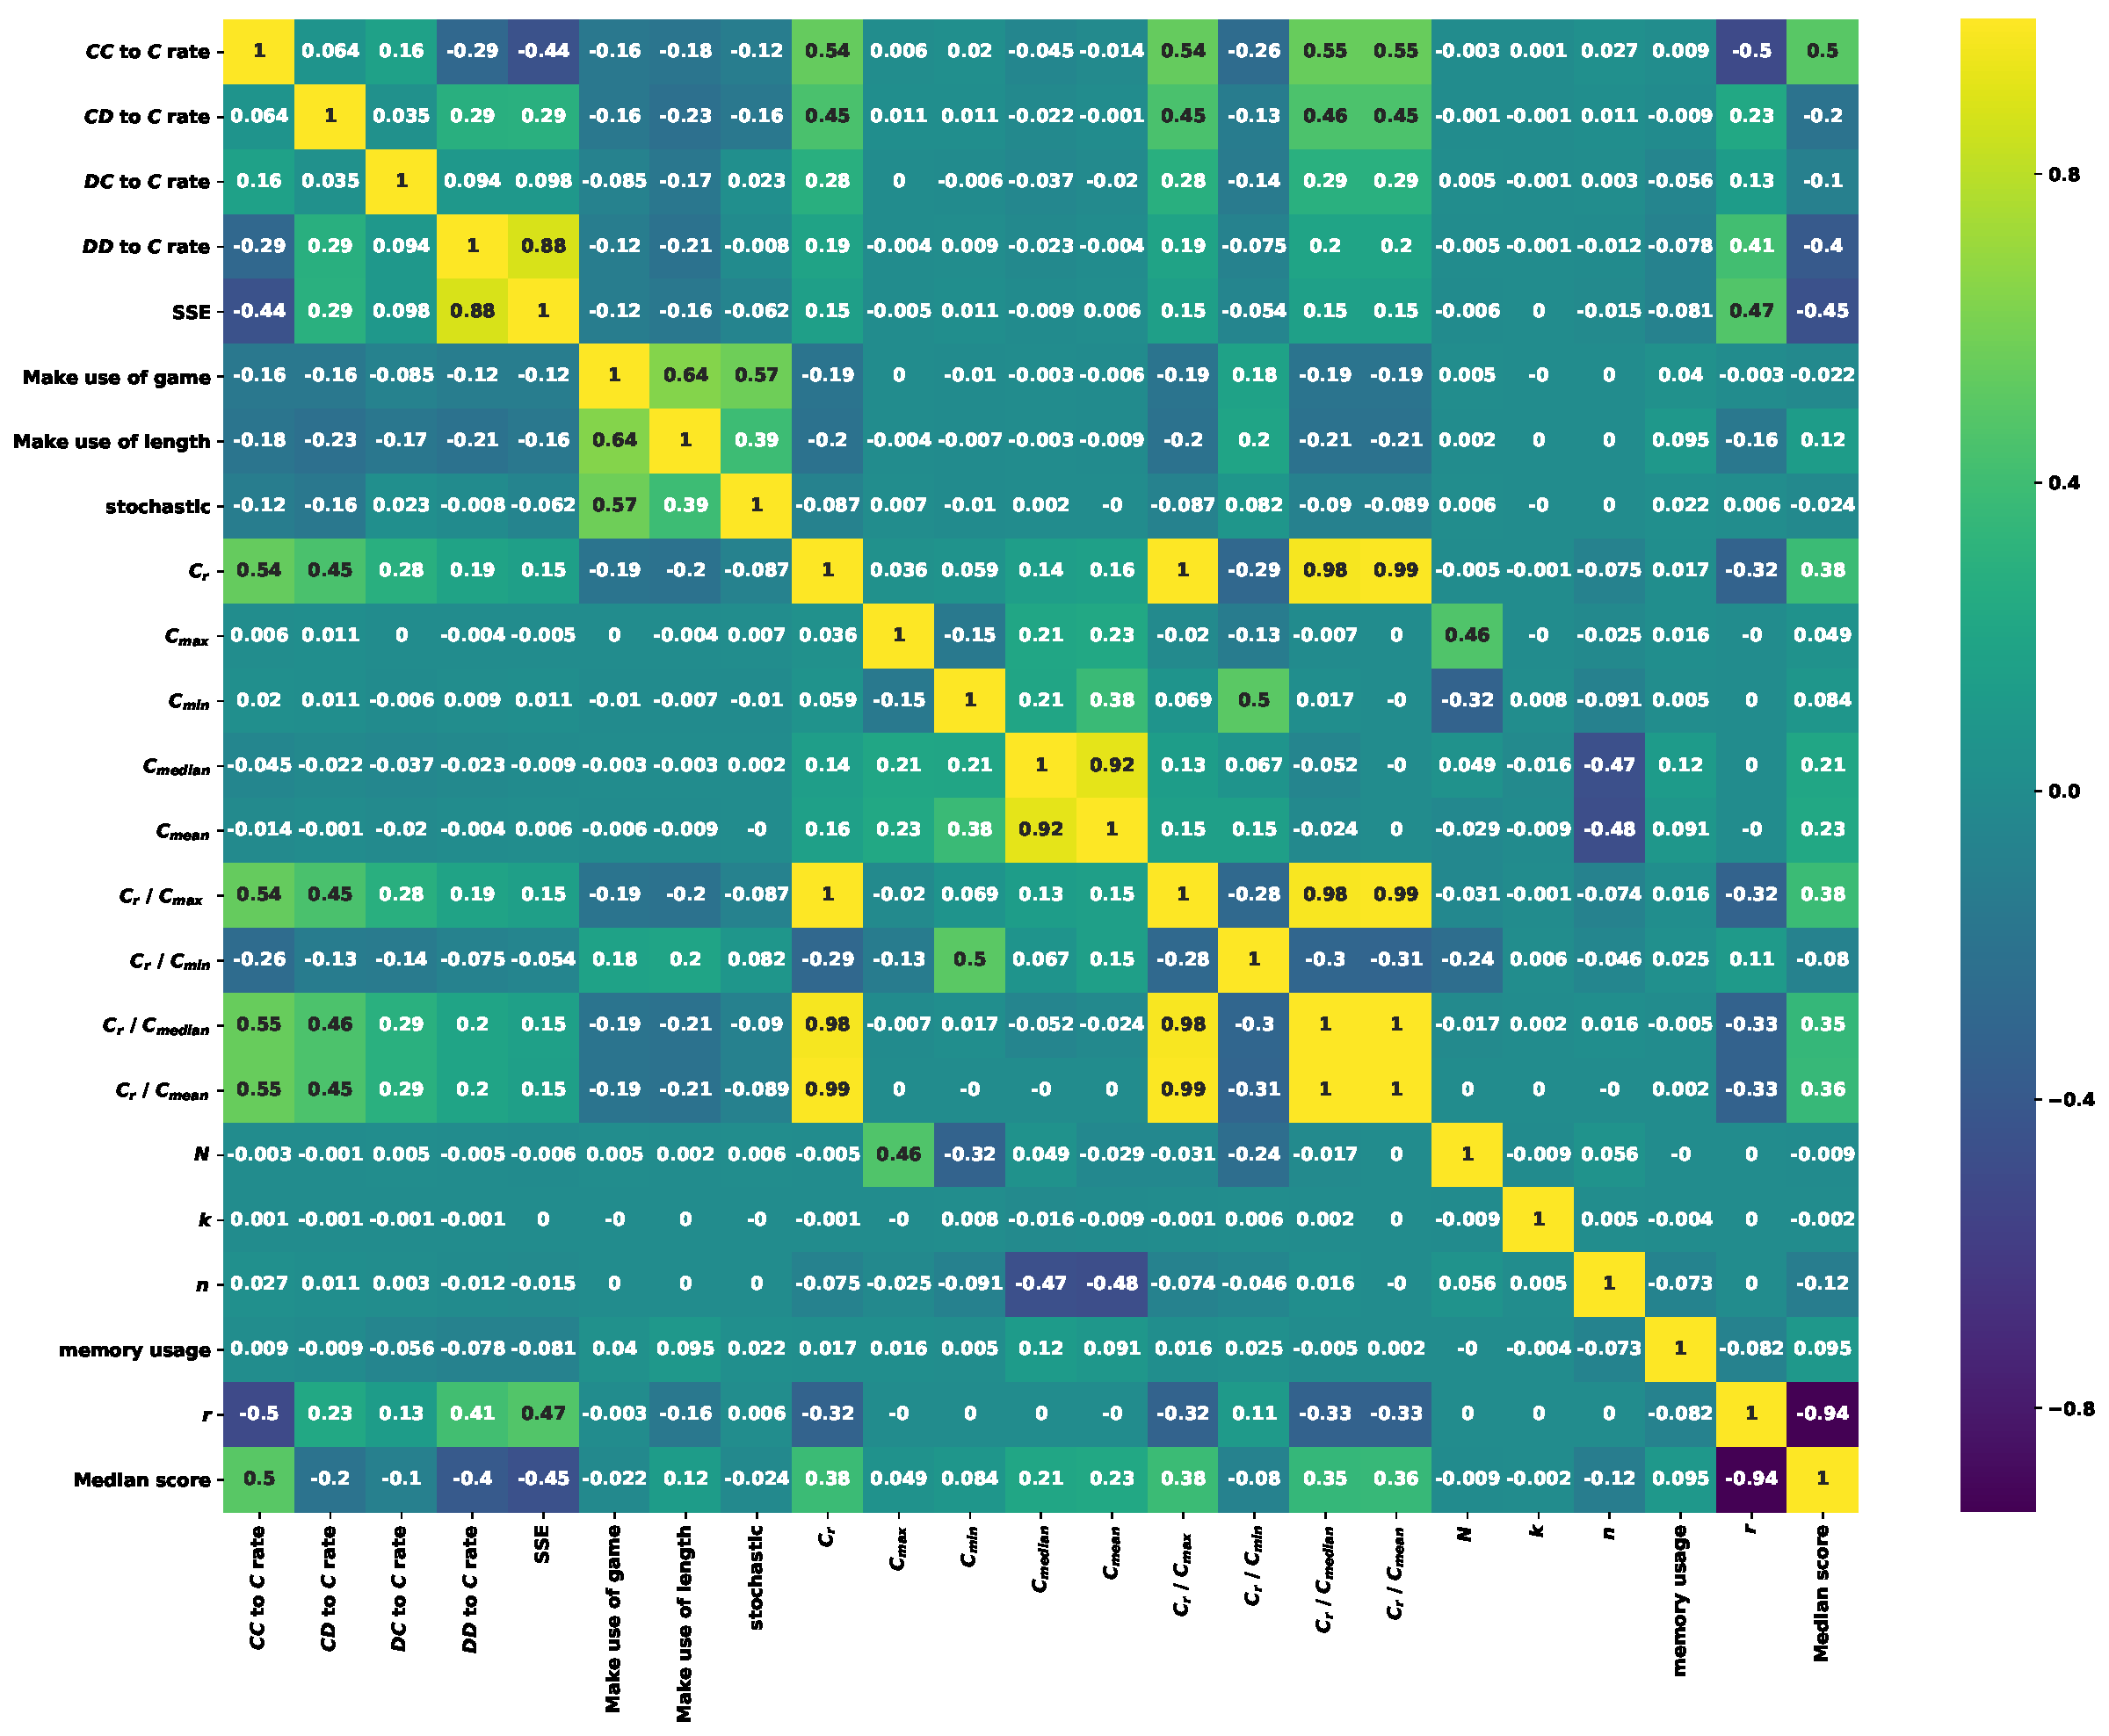
\includegraphics[width=.75\linewidth]{../images/standard_correlation_plot.pdf}
        \end{center}
        \caption{Correlation coefficients of measures in Table~\ref{table:manual_measures}
        for standard tournaments}
\end{figure}
\begin{figure}[!htbp]
    \begin{center}
        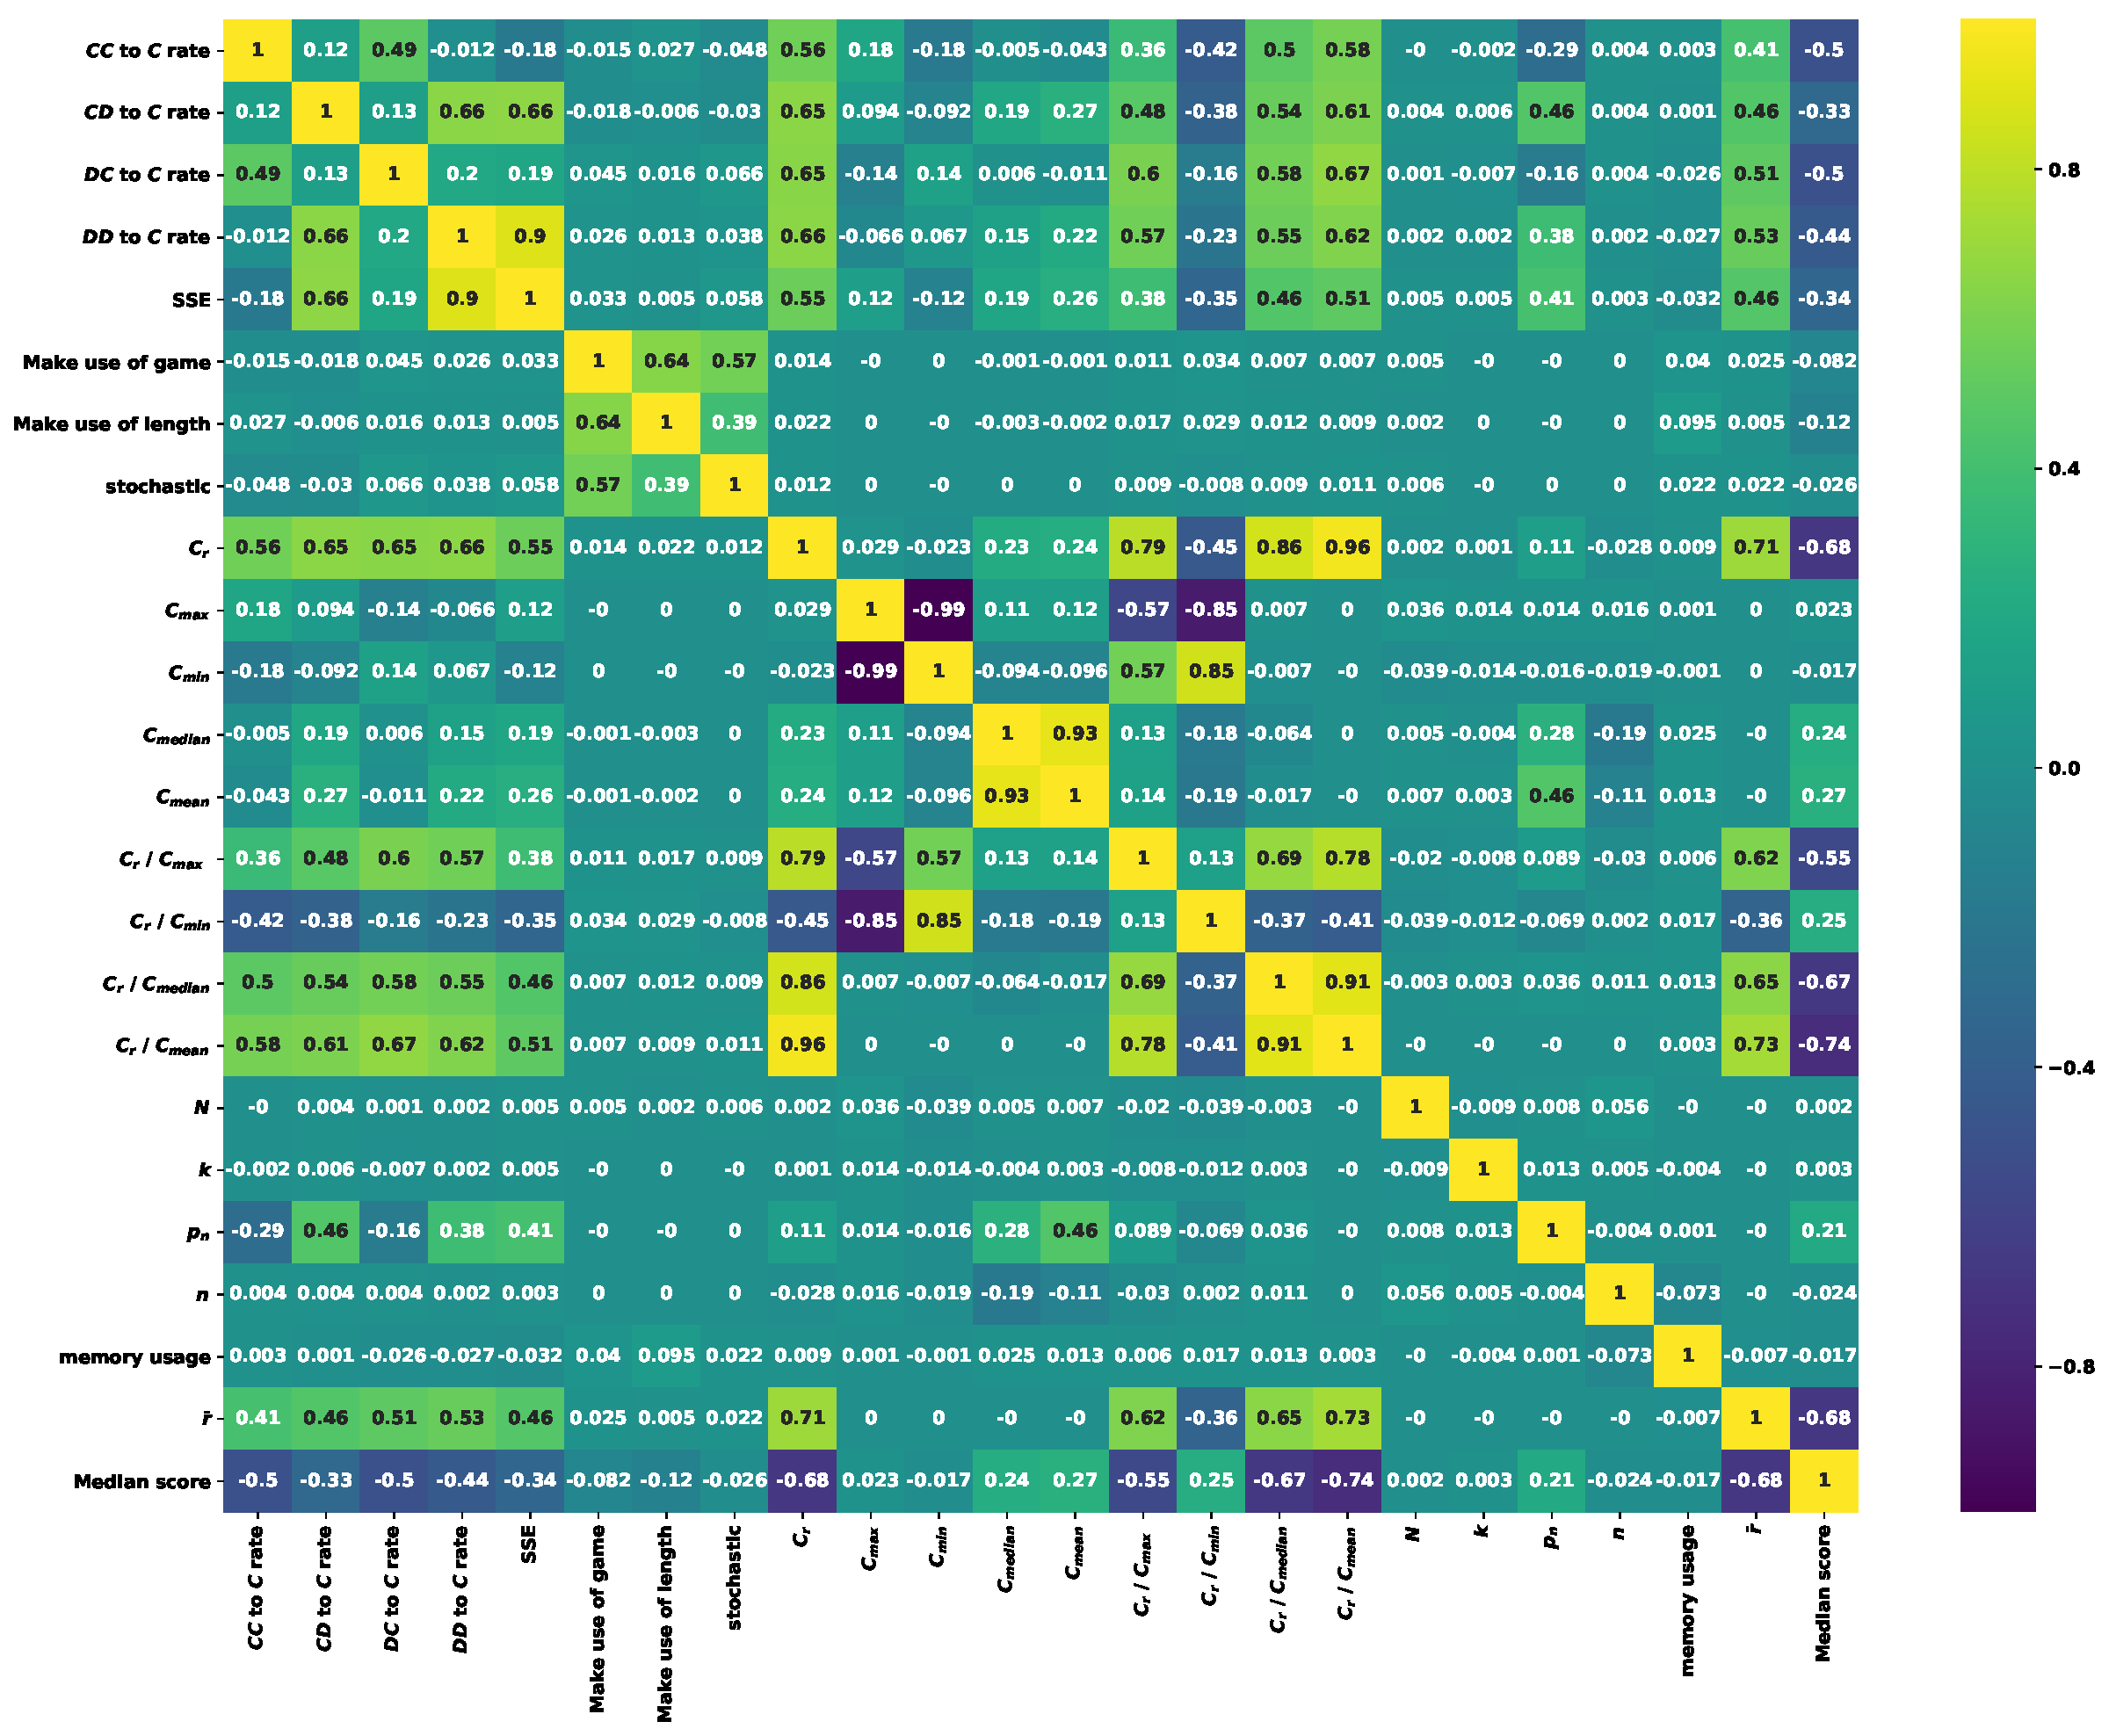
\includegraphics[width=.75\linewidth]{../images/noise_correlation_plot.pdf}
    \end{center}
    \caption{Correlation coefficients of measures in Table~\ref{table:manual_measures}
    for noisy tournaments}
\end{figure}
\begin{figure}[!htbp]
    \begin{center}
        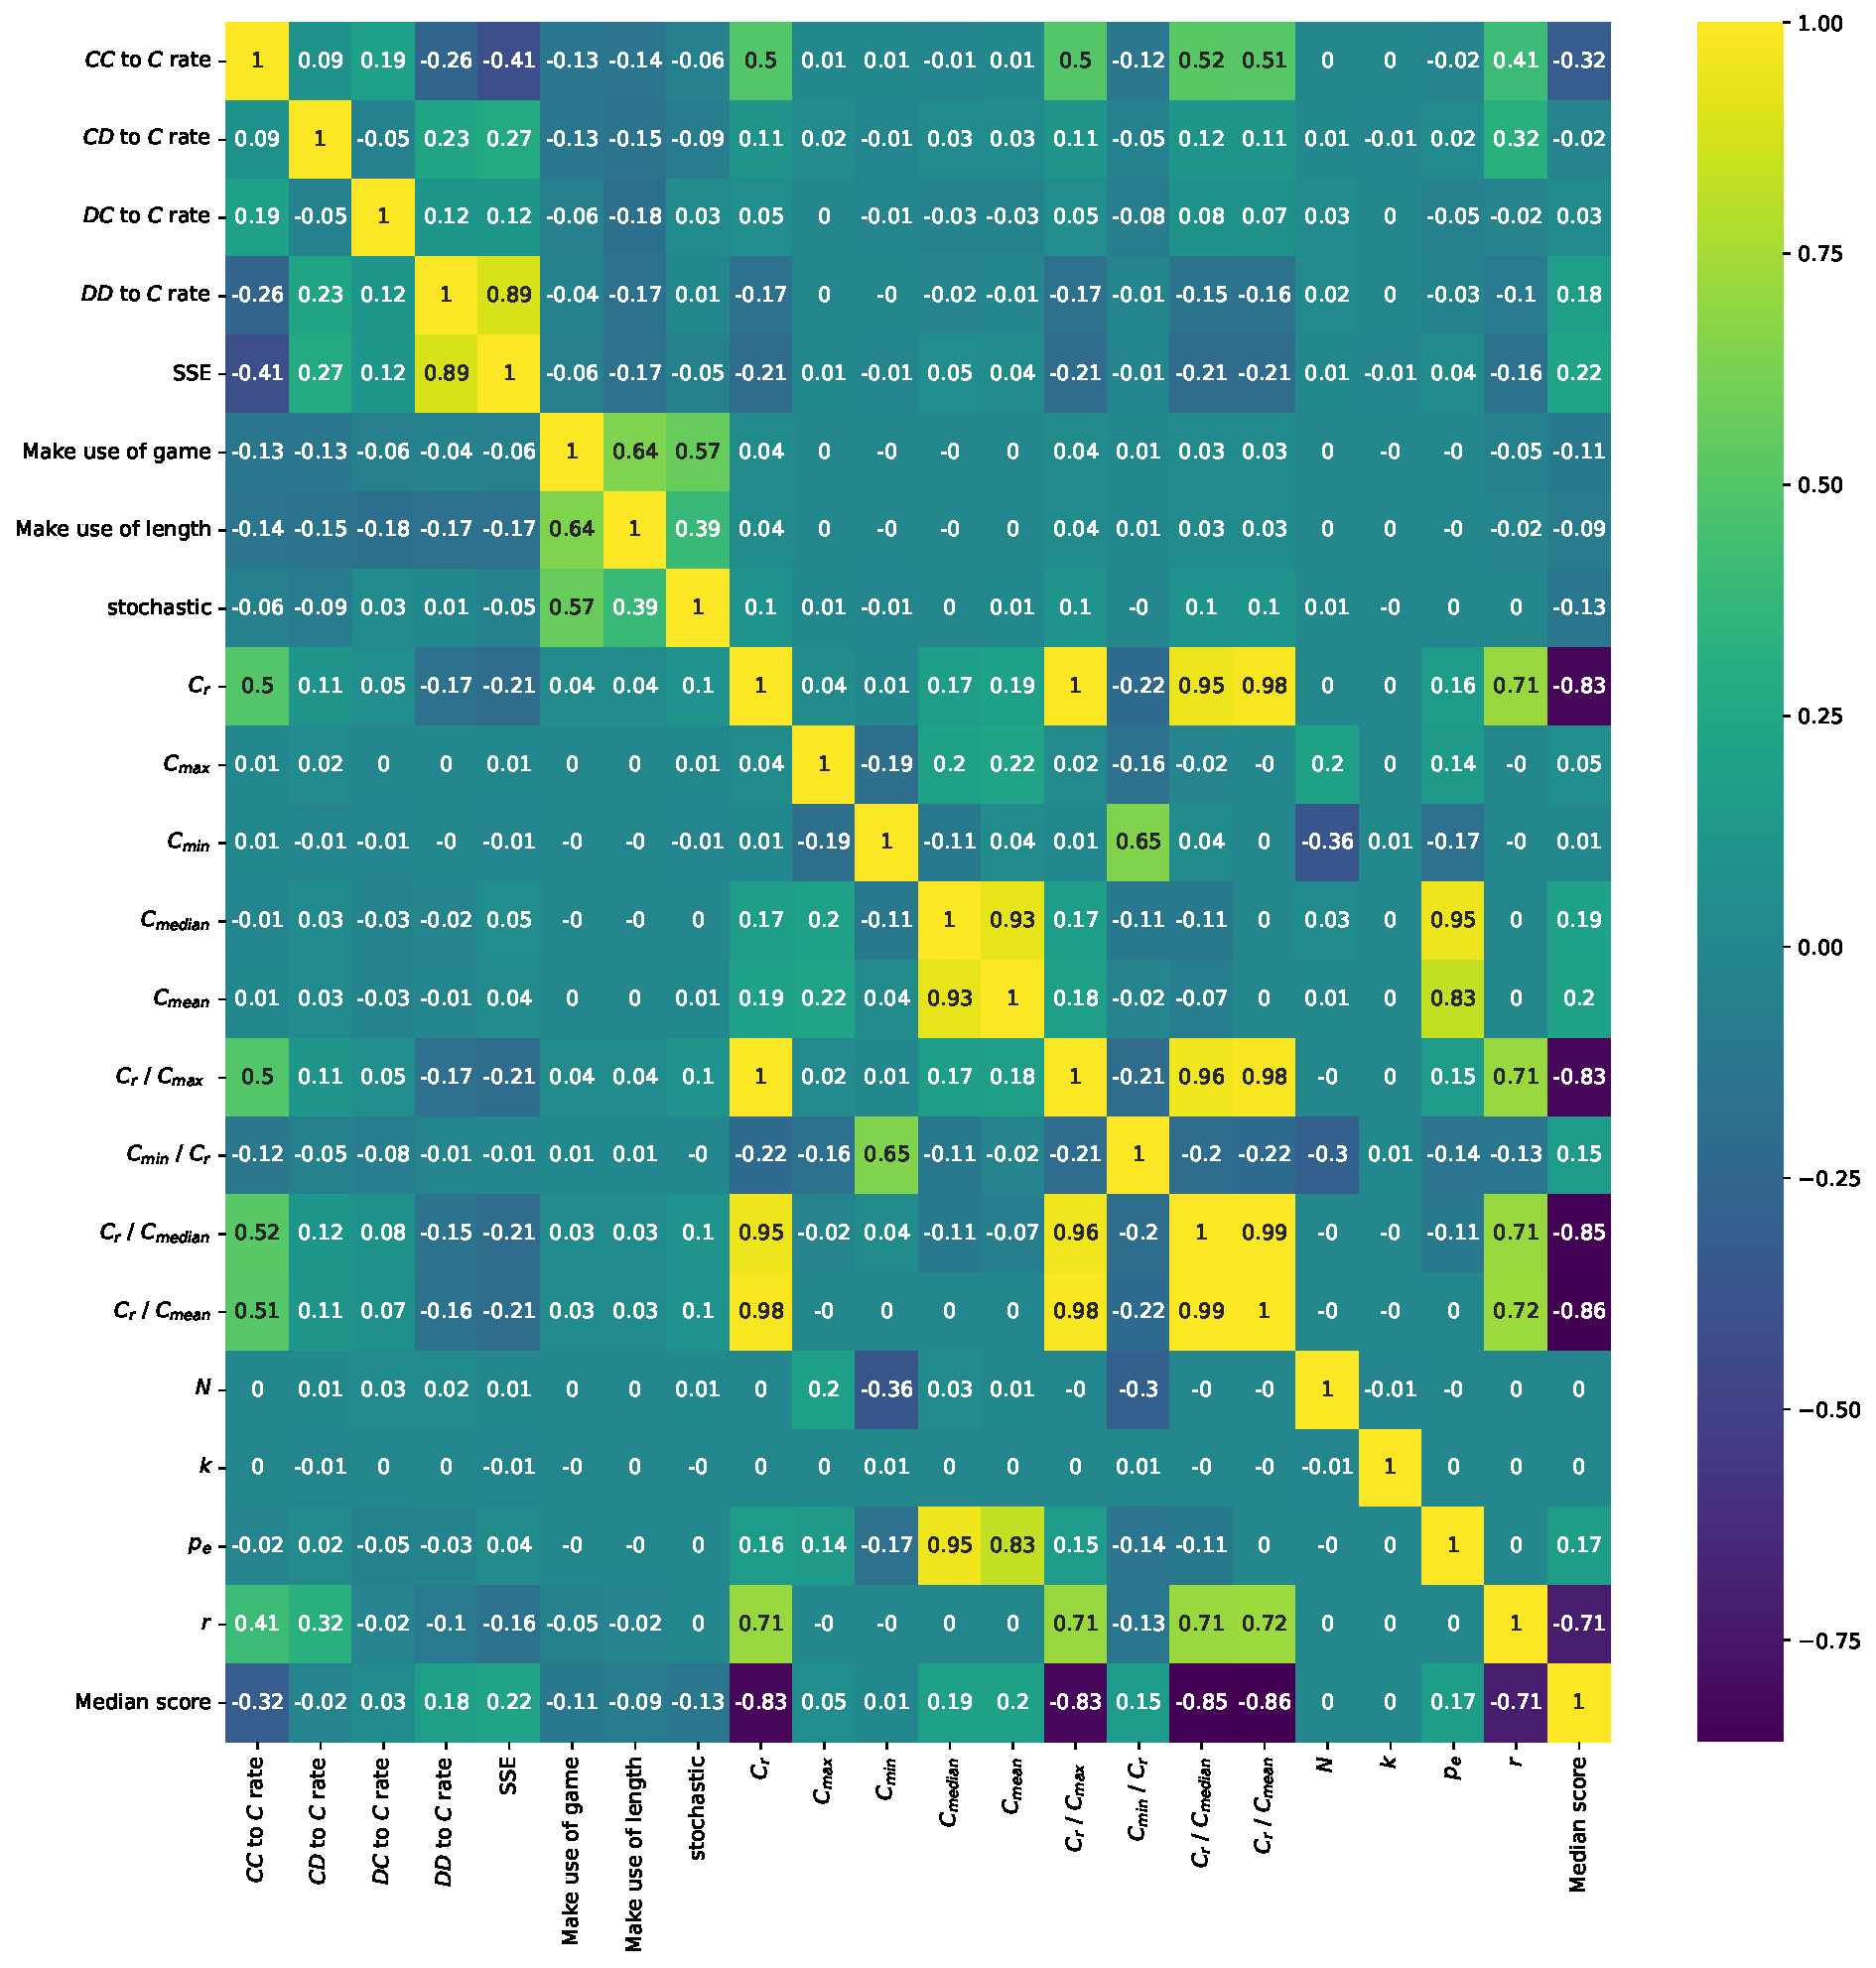
\includegraphics[width=.75\linewidth]{../images/probend_correlation_plot.pdf}
    \end{center}
    \caption{Correlation coefficients of measures in Table~\ref{table:manual_measures}
    for probabilistic ending tournaments}
\end{figure}
\begin{figure}[!htbp]
    \begin{center}
        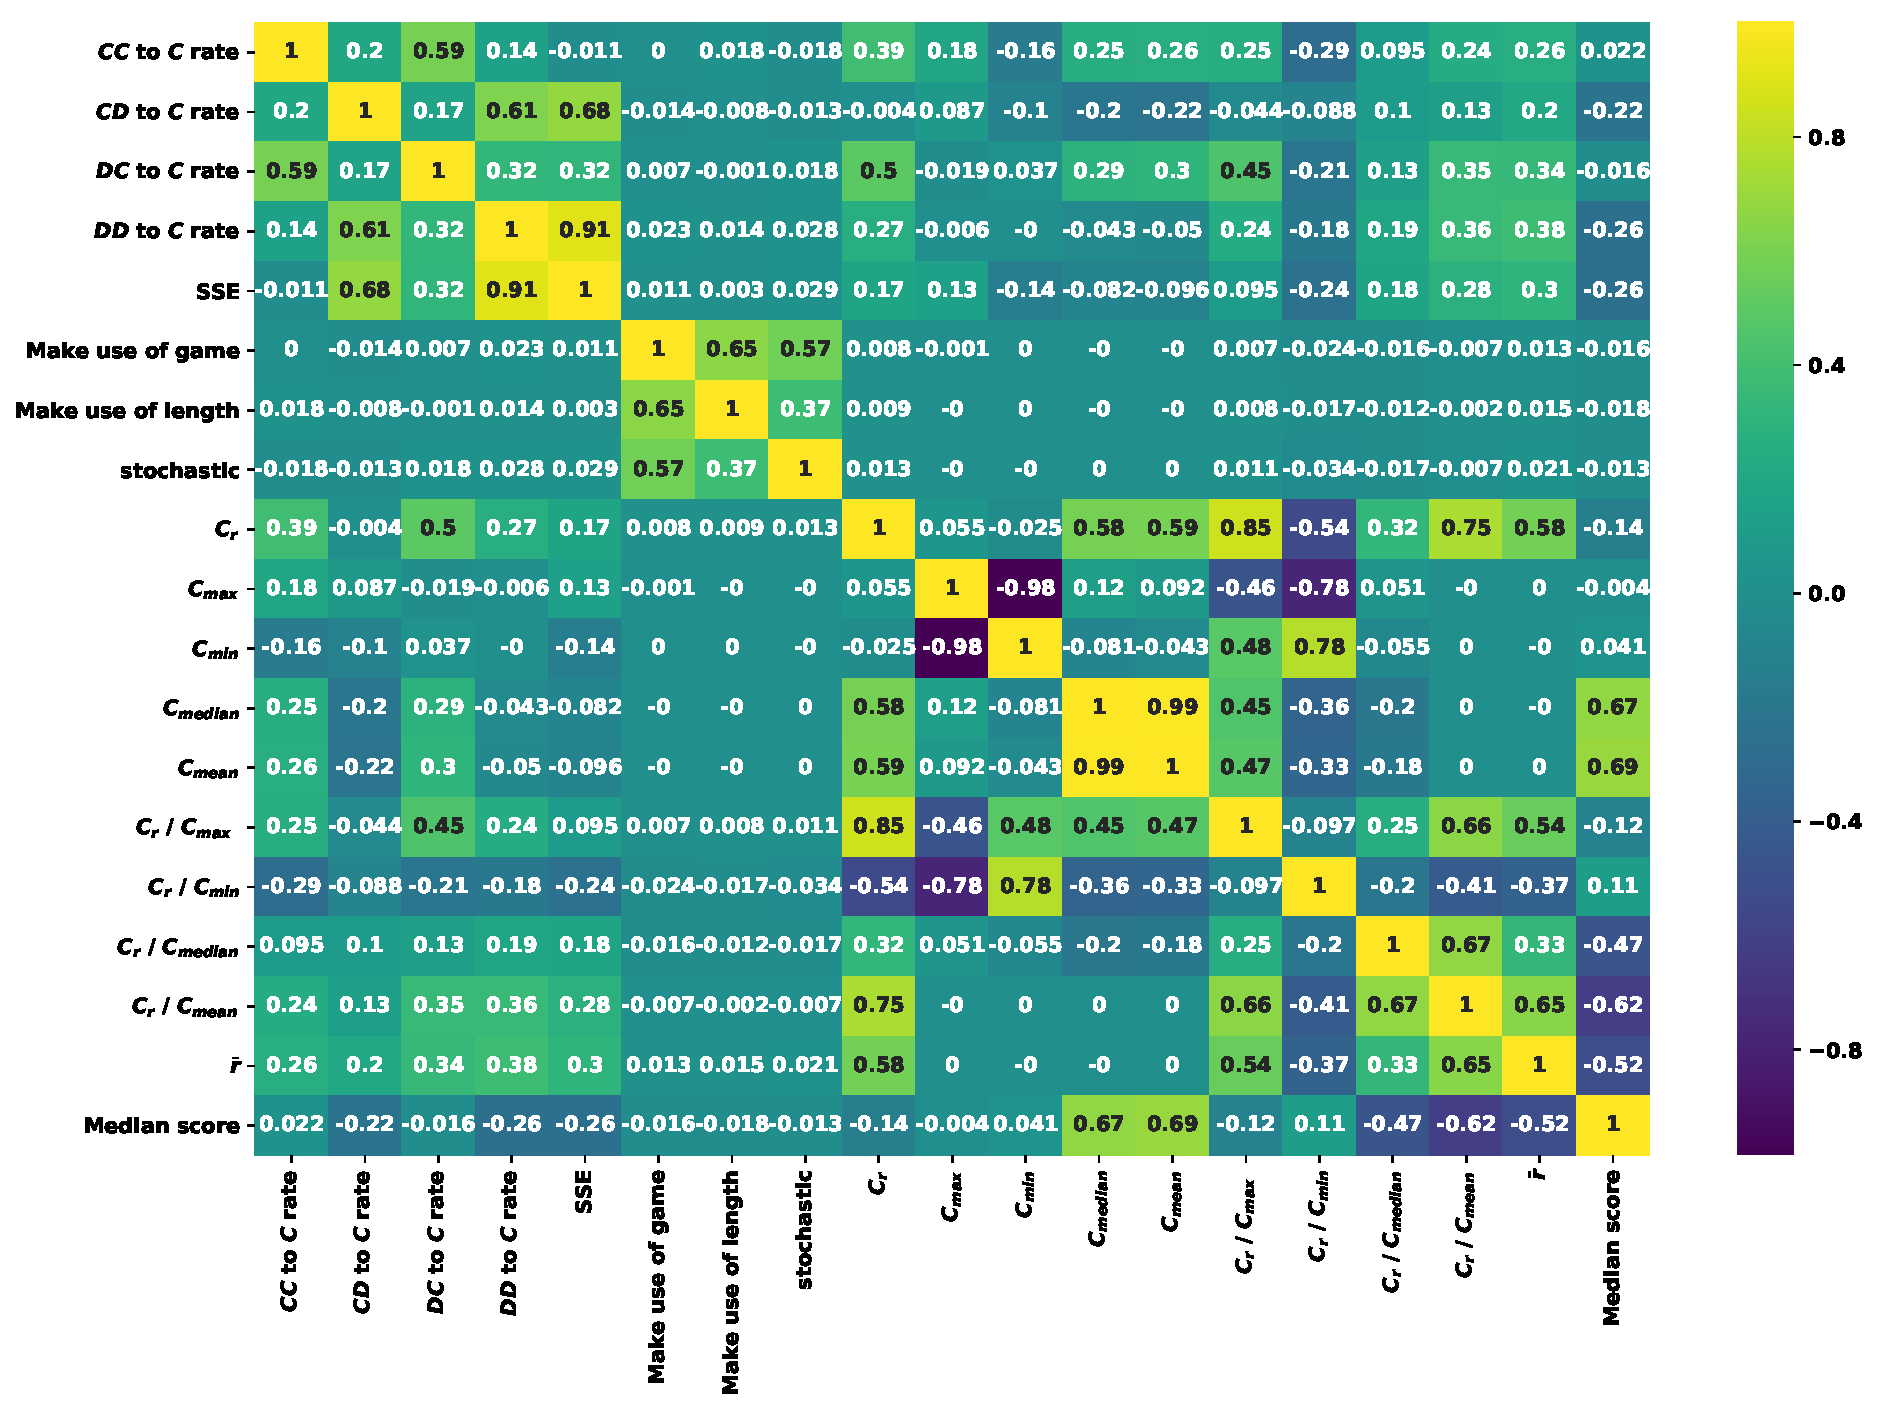
\includegraphics[width=.75\linewidth]{../images/probend_noise_correlation_plot.pdf}
    \end{center}
    \caption{Correlation coefficients of measures in Table~\ref{table:manual_measures}
    for noisy probabilistic ending tournaments}
\end{figure}

\end{document}